% Arquivo principal para trabalhos acadêmicos da UDESC - Joinville

% abnTeX2: Modelo de Trabalho Academico em conformidade com 
% ABNT NBR 14724:2011: Informacao e documentacao - Trabalhos academicos -
% Apresentacao

% Edited by: Eduardo H. Couto
% e-mail: ehcouto@hotmail.com
% ------------------------------------------------------------------------
% ------------------------------------------------------------------------

\documentclass[
	12pt,				% tamanho da fonte
	openright,			% capítulos começam em pág ímpar (insere página vazia caso preciso)
	oneside,			% para impressão em verso e anverso. Oposto a oneside
	a4paper,			% tamanho do papel. 
	chapter=TITLE,		% títulos de capítulos convertidos em letras maiúsculas
	%section=TITLE,		% títulos de seções convertidos em letras maiúsculas
	%subsection=TITLE,	% títulos de subseções convertidos em letras maiúsculas
	%subsubsection=TITLE,% títulos de subsubseções convertidos em letras maiúsculas
	% -- opções do pacote babel --
	english,			% idioma adicional para hifenização
	brazil,				% o último idioma é o principal do documento
	]{./Data/udesc}

\usepackage{./Data/udescsty}
\usepackage{color,graphicx}
\usepackage{multirow}
\usepackage[table,xcdraw]{xcolor}
\usepackage{lscape}
\usepackage{listings}
\usepackage{float}
\usepackage{./Data/jslistings}

\lstset{literate=
	{á}{{\'a}}1 {é}{{\'e}}1 {í}{{\'i}}1 {ó}{{\'o}}1 {ú}{{\'u}}1
	{Á}{{\'A}}1 {É}{{\'E}}1 {Í}{{\'I}}1 {Ó}{{\'O}}1 {Ú}{{\'U}}1
	{à}{{\`a}}1 {è}{{\`e}}1 {ì}{{\`i}}1 {ò}{{\`o}}1 {ù}{{\`u}}1
	{À}{{\`A}}1 {È}{{\'E}}1 {Ì}{{\`I}}1 {Ò}{{\`O}}1 {Ù}{{\`U}}1
	{ä}{{\"a}}1 {ë}{{\"e}}1 {ï}{{\"i}}1 {ö}{{\"o}}1 {ü}{{\"u}}1
	{Ä}{{\"A}}1 {Ë}{{\"E}}1 {Ï}{{\"I}}1 {Ö}{{\"O}}1 {Ü}{{\"U}}1
	{â}{{\^a}}1 {ê}{{\^e}}1 {î}{{\^i}}1 {ô}{{\^o}}1 {û}{{\^u}}1
	{Â}{{\^A}}1 {Ê}{{\^E}}1 {Î}{{\^I}}1 {Ô}{{\^O}}1 {Û}{{\^U}}1
	{Ã}{{\~A}}1 {ã}{{\~a}}1 {Õ}{{\~O}}1 {õ}{{\~o}}1
	{œ}{{\oe}}1 {Œ}{{\OE}}1 {æ}{{\ae}}1 {Æ}{{\AE}}1 {ß}{{\ss}}1
	{ű}{{\H{u}}}1 {Ű}{{\H{U}}}1 {ő}{{\H{o}}}1 {Ő}{{\H{O}}}1
	{ç}{{\c c}}1 {Ç}{{\c C}}1 {ø}{{\o}}1 {å}{{\r a}}1 {Å}{{\r A}}1
	{€}{{\euro}}1 {£}{{\pounds}}1 {«}{{\guillemotleft}}1
	{»}{{\guillemotright}}1 {ñ}{{\~n}}1 {Ñ}{{\~N}}1 {¿}{{?`}}1
}

% ---
% Informações de dados para CAPA e FOLHA DE ROSTO
% ---
\titulo{\textbf{Agil It} \\ Sistema Gerenciador de Ordens de Manutenção de Equipamento para a Indústria de Alimentos}
%\subtitulo{Sistema Gerenciador de Ordens de Manutenção de Equipamento}
\autor{Julio Cesar Thomazelli Junior \\ Lucas Matheus da Silva Gonçalves \\ Márcio Henrique Meier}
\local{Jaraguá do Sul, SC}
\data{2020}
\fulldata{09 de Junho de 2019}
\orientador{Msc. Tathiana Duarte do Amarante}
\instituicao{FACULDADE DE TECNOLOGIA SENAI JARAGUÁ DO SUL}
\tipodoc{Dissertação}
\curso{Graduação tecnológica em sistemas para internet}
\area{Gerenciamento de Ordens de Manutenção}
\preambulo{Trabalho de Conclusão de Curso apresentado à Faculdade de Tecnologia SENAI Jaraguá do Sul como requisito parcial para obtenção do título de Tecnologo em Sistemas para Internet}
% ---

% ----
% Início do documento
% ----
\begin{document}
% ----------------------------------------------------------
% ELEMENTOS PRÉ-TEXTUAIS
% ----------------------------------------------------------
% Retira espaço extra obsoleto entre as frases.
\frenchspacing 

% \pretextual

% ---
% Capa
% ---
\imprimircapa
% ---

% ---
% Folha de rosto
% (o * indica que haverá a ficha bibliográfica)
% ---
\imprimirfolhaderosto*
% ---

% ---
% Inserir a ficha bibliografica
% ---

% Isto é um exemplo de Ficha Catalográfica, ou ``Dados internacionais de
% catalogação-na-publicação''. Você pode utilizar este modelo como referência. 
% Porém, provavelmente a biblioteca da sua universidade lhe fornecerá um PDF
% com a ficha catalográfica definitiva após a defesa do trabalho. Quando estiver
% com o documento, salve-o como PDF no diretório do seu projeto e substitua todo
% o conteúdo de implementação deste arquivo pelo comando abaixo:
%
% \begin{fichacatalografica}
%     \includepdf{fig_ficha_catalografica.pdf}
% \end{fichacatalografica}
%\begin{fichacatalografica}
%	\vspace*{\fill}					% Posição vertical
%	\hrule							% Linha horizontal
%	\begin{center}					% Minipage Centralizado
%	\begin{minipage}[c]{12.5cm}		% Largura
%	
%	\imprimirautor
%	
%	\hspace{0.5cm} \imprimirtitulo  / \imprimirautor. --
%	\imprimirlocal, \imprimirdata-
%	
%	
%	\hspace{0.5cm} \imprimirorientadorRotulo~\imprimirorientador\\
%	
%	\hspace{0.5cm}
%	\parbox[t]{\textwidth}{\imprimirtipotrabalho~--~\imprimirinstituicao,
%	\imprimirdata.}\\
%	
%	
%	\end{minipage}
%	\end{center}
%	\hrule
%\end{fichacatalografica}
% ---


% ---
% Inserir errata (Se necessário)
% ---
%\begin{errata}
%Elemento opcional da \citeonline[4.2.1.2]{NBR14724:2011}. Exemplo:
%
%\vspace{\onelineskip}
%
%FERRIGNO, C. R. A. \textbf{Tratamento de neoplasias ósseas apendiculares com
%reimplantação de enxerto ósseo autólogo autoclavado associado ao plasma
%rico em plaquetas}: estudo crítico na cirurgia de preservação de membro em
%cães. 2011. 128 f. Tese (Livre-Docência) - Faculdade de Medicina Veterinária e
%Zootecnia, Universidade de São Paulo, São Paulo, 2011.
%
%\begin{table}[htb]
%\center
%\footnotesize
%\begin{tabular}{|p{1.4cm}|p{1cm}|p{3cm}|p{3cm}|}
%  \hline
%   \textbf{Folha} & \textbf{Linha}  & \textbf{Onde se lê}  & \textbf{Leia-se}  \\
%    \hline
%    1 & 10 & auto-conclavo & autoconclavo\\
%   \hline
%\end{tabular}
%\end{table}
%
%\end{errata}
% ---

% ---
% Inserir folha de aprovação
% ---

% Isto é um exemplo de Folha de aprovação, elemento obrigatório da NBR
% 14724/2011 (seção 4.2.1.3). Você pode utilizar este modelo até a aprovação
% do trabalho. Após isso, substitua todo o conteúdo deste arquivo por uma
% imagem da página assinada pela banca com o comando abaixo:
%
% \includepdf{folhadeaprovacao_final.pdf}
%
% ---

% ---
% Dedicatória
% ---
% ---

% ---
% Agradecimentos
% ---
% ---

% ---
% Epígrafe
% ---
% ---

% ---
% RESUMOS
% ---

% resumo em português
% resumo em inglês
% ---
% inserir lista de ilustrações
% ---
\pdfbookmark[0]{\listfigurename}{lof}
\listoffigures*
\cleardoublepage
% ---

% ---
% inserir lista de tabelas
% ---
%\pdfbookmark[0]{\listtablename}{lot}
%\listoftables*
%\cleardoublepage
% ---

% ---
% inserir lista de abreviaturas e siglas
% ---
\begin{siglas}
  \item[MVP]      Minimum Viable Product
  \item[API]      Application Programming Interface
  \item[ORM]      Object-Relational Mapping
  \item[OM]		  Ordem de Manutenção
  \item[ERP]      Enterprise Resource Planning
  \item[SAP]	  Systeme, Anwendungen und Produkte in der DatenverarbeitungERP
  \item[WEB]	  Internet
  \item[UC]		  Unidade Curricular
  \item[JWT]	  Json Web Token
\end{siglas}
% ---


% ---
% inserir o sumario
% ---
\pdfbookmark[0]{\contentsname}{toc}
\tableofcontents*
\cleardoublepage
% ---

\textual
% ---

% ----------------------------------------------------------
% ELEMENTOS TEXTUAIS
% ----------------------------------------------------------
\chapter{Introdução ao Documento}

{A faculdade SENAI (Serviço Nacional de Aprendizagem Industrial) \footnote{\url{http://sc.senai.br/pt-br/faculdade-senai-jaragua-do-sul}}  visa sistematizar os conhecimentos adquiridos pelos estudantes durante o decorrer do curso, como também, oferecer vivência  prática-profissional mediante a aplicação dos conhecimentos em situações reais. Além disso, busca  propiciar ao estudante o contato com o universo acadêmico da iniciação científica, através da implantação do \textit{Projeto Integrador}, que tem exatamente essas características em locais que está sendo implantado. Portanto o Senai está em parceria com a empresa Duas Rodas desenvolvendo este projeto. }



A empresa Duas Rodas possui sua sede em Jaraguá do Sul, Santa Catarina e tem como principal ramo a indústria de alimentos \footnote{\url{ https://www.duasrodas.com/}}. Para a execução de suas tarefas diárias, seus funcionários contam com o auxílio direto de máquinas de pequeno, médio e grande porte, e sabe-se que esses equipamentos necessitam, de manutenção preditiva e corretiva  de tempos em tempos. Para tanto, se faz necessário ajustes adequados e rápidos para que não haja baixa produtividade e consequentemente uma redução em seus proventos.

Esses equipamentos precisam passar por uma série de cuidados e estar em bom estado para o uso dos seus colaboradores. Portanto, é de extrema importância para empresa Duas Rodas ter um controle e um bom fluxo de manutenções desses equipamentos, de modo a não haver uma inatividade desnecessária, e quando necessário a manutenção, esta seja rápida e eficiente.

% CAP 1.1
% ---
\section{Tema}
% ---
O projeto consiste no desenvolvimento de um sistema de ordem de manutenção de máquinas e equipamentos que busca minimizar os trâmites burocráticos e demorados que hoje está sendo utilizado.

% CAP 1.2
% ---
\section{Objetivo do Projeto}
% ---
O objetivo do projeto é que a empresa alimentícia Duas Rodas consiga digitalizar
o fluxo de manutenção de seus equipamentos não afetando a demanda de serviço e facilitando a execução das OMs que encontra-se em fila, reduzindo assim a utilização excessiva de papel.

% CAP 1.3
%---
\section{Delimitação do Problema}
%---
Atualmente a empresa Duas Rodas gera ordens de manutenção no SAP e imprime um formulário padrão. Esse formulário é passado para o manutentor, que realizará a manutenção e preencherá todos os campos necessários do formulário. Após a finalização da manutenção, os usuários responsáveis assinam esse formulário para comprovar que o problema foi resolvido. Após as assinaturas, o formulário é enviado a um usuário administrativo que irá aprovar e enviar ao SAP.
% ---

% CAP 1.4
% ---
\section{Justificativa da Escolha do Tema}
% ---
Este projeto surgiu por meio da deficiência encontrada nos setores de manutenção da empresa, onde os mesmos relataram os problemas e dificuldades na execução de manutenção nas máquinas e equipamentos. Desta forma, em parceria com a instituição de ensino SENAI e o Curso de Sistemas para Internet de Jaraguá do Sul, resolveu-se implementar no Projeto Integrador, o desenvolvimento de um Software baseado no gerenciamento de ordens de manutenção.

% CAP 1.5
% ---


% CAP 1.6
% ---
\section{Método de Trabalho}
% ---
Para o desenvolvimento do projeto será utilizado a metodologia SCRUM no formato MVP (Produto Mínimo Viável).

O Scrum, criado em 1993 por Ken Schwaber e Jeff Sutherland, tem a origem de seu nome no “jogo de rúgbi e se refere à maneira como um time trabalha junto para avançar com a bola no campo. Alinhamento cuidado, unidade de propósito, clareza de objetivo, tudo se unindo \cite{rocha2015metodologia}.
A metodologia SCRUM consiste em quebrar o sistema em várias partes pequenas e fazer entregas a cada ciclo, que normalmente possuem de 1 a 2 semanas.
Enquanto o formato MVP prega o desenvolvimento de algo com o menor investimento possível, a fim da validação da ideia ou conceito utilizado.

% CAP 1.7
% ---
\section{Organização do Trabalho}
% ---
Este documento se dará da seguinte maneira: será feito uma descrição geral do sistema, os requisitos do sistema, a análise e design e a implementação do sistema.

% CAP 1.8
% ---
\section{Glossário}
SCRUM:		Metodologia ágil de desenvolvimento de projetos.

MVP:		Produto com o mínimo valor possível, visado para validação da ideia do projeto.

API:		Interface para comunicação entre diferentes aplicações.

ORM:		Tecnologia que auxilia o gerenciamento do banco de dados através da modelagens de classes.

Express:	Tecnologia que abstrai requisições web.

Sequelize:	Biblioteca de ORM para bancos relacionais, incluindo SQL Server.

Feedback:	Retorno a um acontecimento.

Software:	Programa de computador.

UC:			Unidade Curricular.

EAP:		Estrutura Analítica do Projeto.

PMBOK:      Conhecimento em Gerenciamento de Projetos.

% ---
\chapter{Fundamentação Teórica}

\section{Sistemas Computacionais}

Os sistemas computacionais tomaram conta da sociedade atual, o uso de tecnologias computacionais vem tendo muito espaço na comunidade, seja fazendo uso de um computador pessoal, smartphone ou um tablet. Sendo assim, tais dispositivos foram criado essencialmente para satisfazer as necessidades das empresas de forma a garantir e resolver seus problemas organizacionais, ou seja, a criação de uma ferramenta que possa armazenar e cruzar dados e informações sem que sejam necessárias pilhas de papéis. Estes sistemas garantem às empresas a possibilidade de atingir mercados em locais mais distantes. \cite{MATTIOLI2020}.

Destaca-se, que o sistema da informação é um tipo especializado de sistema, que pode ser definido de várias formas. Com isso, pode-se entender que sistemas são séries de elementos ou componentes inter-relacionados que coletam entrada de dados, manipulando-os, processando-os, disseminando a saída dos dados e informações, fornecendo assim um mecanismo de \textit{feedback}. \cite{STAIR2008}.

Atualmente a palavra \textbf{sistema} é mal utilizada, usa-se de forma indiscriminada e sem qualquer tipo de fundamento, ou ainda, é usada para expressar determinadas situações dentro de um software, principalmente nos meios empresariais conforme explica \cite{ROSSINI2006}.

Diante disso, é importante conceituar dados, sendo estes como fatos básicos, por exemplo, o nome e a quantidade de horas trabalhadas em uma semana de um funcionário, quantidade de peça em estoque ou pedidos. Importante mencionar que as informações são compostas por um conjunto de fatos organizados de modo a terem valor adicional, além do valor dos fatos propriamente ditos. Portanto, quando dados são organizados ou alcançados de maneira significativa, se transformam em informações. \cite{STAIR2008}.

Conforme informações acima dispostas, apesar de o termo sistema estar muito difundido e utilizado muitas vezes de forma leviana, seu significado é bastante preciso. Um sistema é um conjunto de elementos que trabalham de forma integrada a atingir uma ou mais finalidades.
Para que o sistema funcione corretamente, é necessário transformar dados em informações de forma que seus objetivos sejam alcançados, desde a finalidade única de cada elemento até a totalidade das funcionalidades integradas do mesmo.

No próximo capitulo será abordado a computação verde.

\section{Computação Verde}

Computação ou TI Verde é um conjunto de iniciativas de investimento na implantação, uso e gerenciamento que tem a finalidade de minimizar o impacto negativo ambiental na área de tecnologia da informação. \cite{CQP_MMD_2020}.

O investimento de capital em computação verde é composto por três dimensões: estrutural, humano e relacional.
O capital estrutural refere-se a infraestrutura da TI que engloba \textit{hardware}, \textit{software}, redes e tecnologia da informação. O capital humano é a capacidade e experiência dos profissionais de TI a respeito de conservação de energia em tecnologia e desenvolvimento pessoal com capacidades em TI verde, obtida através de treinamento e estudos. Por último, o capital relacional envolve o gerenciamento da TI verde e a relação das organizações com seus parceiros e usuários, implementando conceitos de proteção ambiental em produtos e serviços. \cite{CQP_MMD_2020}.

Com isso, a adoção das práticas de TI verde propicia uma operação mais sustentável às organizações, gerando economia com energia, papel, água, transporte, espaço físico, manutenção e descarte, proporcionando assim valor tanto para a organização quanto para a sociedade \cite{TallesMoura2017}.

No próximo capitulo será abordado o planejamento e gerenciamento de projetos de software.

\section{Planejamento e Gerenciamento de Projetos de Software}

Um projeto é um empreendimento temporário que objetiva criar um produto, resultado ou serviço único, que no caso de projeto de software é o sistema em funcionamento \cite{Julia_Mara_2018}.

Os projetos de software apresentam particularidades principalmente por desenvolver produtos incompreensíveis e pela dificuldade do seu gerenciamento, além da falta de comunicação entre os gerentes/desenvolvedores e os clientes/usuários \cite{Prado1999}. As etapas de desenvolvimento seguem um ciclo de vida com fases próprias, tais como a especificação de requisitos, análise, projeto, implementação, testes e implantação \cite{Ralf_Teresa_Erica2018}.

A competitividade e os avanços tecnológicos provocaram um aumento na exigência de qualidade e na complexidade de decisões administrativas. Para obter êxito em um projeto é necessário planejar e gerenciar com eficiência a execução de diversas atividades independentes, pois o grau de risco e incerteza quanto ao sucesso do projeto são elevados \cite{Maria_Isabel_2001}.

Para gerir um projeto, é possível utilizar modelos mais prescritivos como o PMBoK, mais adaptativos como o Scrum ou híbridos.
Os modelos prescritivos possuem uma estrutura formal de elementos do processo como atividades e tarefas, um fluxo de trabalho que descreve como cada um destes elementos deve ocorrer e como eles são relacionados. A busca pela estrutura e a ordem é uma característica importante deste tipo de modelo, que normalmente são compostos por \textit{frameworks} como PMBoK, PRINCE2 e IPMA\cite{Julia_Mara_2018}.
Enquanto os modelos prescritivos presam principalmente pela metodologia e pelo fluxo dos processos, modelos adaptativos como os oriundos do manifesto ágil, são focados na interação entre os usuários no processo de construção do produto através de uma abordagem iterativa e adaptativa\cite{Julia_Mara_2018}.
Os métodos ágeis possuem valores fundamentais, que foram definidos no manifesto ágil, de 2001:
\begin{itemize}
	\item Indivíduos e interação entre eles mais que processos e ferramentas;
	\item Software em funcionamento mais que documentação abrangente;
	\item Software em funcionamento mais que documentação abrangente;
	\item Responder a mudanças mais que seguir um plano.
\end{itemize}

\begin{figure}[htb]
	\caption{\label{planejamento_21}Planejamento de Projeto}
	\begin{center}
		\includegraphics[scale=0.45]{./Figuras/planejamento_projeto.png}
	\end{center}
	\legend{Fonte: \cite{Maria_Isabel_2001}}
\end{figure}

A figura \ref{planejamento_21} mostra o ciclo de gerenciamento de projetos de software. O controle atua tanto no planejamento quanto no desenvolvimento, proporcionando desvios que originam ações corretivas. Entretanto, a avaliação ao final do projeto, reabastece o planejamento com novos projetos e ideias, prosseguindo assim em ciclo indeterminado. Já os padrões são definidos a partir dos controles e das avaliações para controlar e planejar o decorrer do projeto.

No próximo capitulo será abordado a UML.

\section{UML - \textit{Unified Modeling Language}}
A UML foi desenvolvida com o propósito de fornecer a arquitetos e engenheiros, ferramentas para análise, design e implementação de software, bem como oferecer suporte à modelagem de negócio \cite{gasparini2018driv}. A UML é dividido em dois grupos: estrutural que permite representar a parte estática do sistema e comportamental que permite representar objetos dinâmicos no sistema \cite{silva2018sasml}.

Os modelos estruturais utilizam classes de objetos e seus relacionamento, os relacionamentos importantes que podem ser documentados nesse estágio são os de generalização e composição. Enquanto os modelos dinâmicos mostram as interações entre os objetos do sistema, as interações que podem ser documentadas incluem a sequência de solicitação de serviço feitas pelos objetos e as mudanças de estado que são disparadas por essas interações de objetos \cite{sommerville2011software}.

A figura \ref{Exemplo_UML} representa um modelo de diagrama de classes que aborda uma experiência em um \textit{e-commerce}. Um cliente pode fazer o login na plataforma, inserir, excluir e alterar produtos e finalizar a compra. Cada item do carrinho possui o produto e a quantidade, e o produto possui preço e descrição.
Após finalizar o carrinho a plataforma gera um pedido que gera um pagamento.
\begin{figure}[htb]
	\caption{\label{Exemplo_UML} Exemplo de modelo conceitual especificado em UML}
	\begin{center}
		\includegraphics[scale=0.45]{./Figuras/Exemplo_UML.png}
	\end{center}
	\legend{Fonte: \cite{monica_diagrama}}
\end{figure}

No próximo capitulo será abordado a metodologia ágil de desenvolvimento SCRUM.
\section{SCRUM}
O Scrum, criado em 1993 por Ken Schwaber e Jeff Sutherland, tem a origem de seu nome no jogo de rúgbi e se refere à maneira como um time trabalha junto para avançar com a bola no campo. Tudo se alinha: posicionamento cuidadoso, unidade de propósito, clareza de objetivo, tudo se unindo \cite{rocha2015metodologia}.

O Scrum é um \textit{framework} utilizado em projetos ágeis para o gerenciamento e desenvolvimento de produtos, tendo como foco a entrega de valor de um negócio no menor tempo possível \cite{cruz2013scrum}. Baseia-se em aproveitar a maneira como as equipes trabalham de fato, fornecendo ferramentas para se auto organizarem e otimizarem a velocidade e qualidade do trabalho \cite{sutherland2016scrum}.

Por conta disso, o Scrum vem sendo adotado por organizações de diversos tamanhos e tipos, desde multinacionais à \textit{startups}, de famosas a desconhecidas. É utilizado em projetos de características igualmente diversificadas, projetos críticos de centenas de milhares de dólares e em projetos internos e simples \cite{sabbagh2014scrum}.

No próximo capitulo será abordado a tecnologia GIT.
\section{GIT}
O Git é um sistema de controle de versão (SCM) distribuído e um sistema de gerenciamento de código fonte. Foi projetado e desenvolvido por Linus Torvalds, o criador do Linux \cite{souzagerenciamento}.
O Git permite que uma equipe de desenvolvedores possam trabalhar de forma colaborativa em um projeto sem a preocupação com perda de informação na edição ou criação de arquivos \cite{konnorate2019importancia}.
Apesar de ser distribuído e não depender de um servidor central, normalmente existe um servidor principal chamado de \textit{origin}, a partir dele os desenvolvedores do projeto clonam e trabalham nesse repositório sem necessitar mais da comunicação com o repositório principal até ser necessário sincronizar as mudanças novamente \cite{cunha2018entendendo}.
Enquanto os desenvolvedores trabalham em suas atividades, mudanças paralelas podem ocorrer, resultando em conflitos ao integrar o código. Resolver estes conflitos não é uma tarefa trivial, podendo se tornar custosa ao desenvolvedor. Estes tipos de problemas não possuem uma solução exata, pois existe mais de uma maneira de solucioná-los \cite{cunha2018entendendo}.

No próximo capitulo será abordado a técnica ORM.
\section{ORM - \textit{Object-Relational Mapping}}

ORM é um método de programação para troca de dados entre tipos de sistemas incompatíveis de banco de dados relacionais e linguagem orientada a objetos. A tecnologia ORM constitui um ``banco de dados orientado a objetos virtual'' que consegue lidar internamente com a linguagem de programação \cite{nazario2019detecting}. O seu principal objetivo é reduzir a impedância da programação orientada a objetos na utilização de bancos de dados relacionais, nela, as tabelas do banco de dados são mapeadas em classes e os registros de cada tabela são mapeados em instâncias das classes correspondentes \cite{michalsky2012componentes}, de forma que o objeto não precisa saber nada a respeito do banco de dados e nem o banco de dados ter algum conhecimento em relação ao objeto ou a estrutura de dados da aplicação, toda a conversão é realizada pela ORM \cite{fayyaz2014performance}.
O uso de \textit{frameworks} ORM reduzem significativamente o esforço de não apenas comunicar com o banco de dados mas também de lidar com operações básicas do mesmo, como inserir, atualizar, ler e deletar registros, já que as alterações de objetos são propagas automaticamente aos registros correspondentes na base de dados \cite{nazario2019detecting}.
\chapter{Descrição Geral do Sistema}
%---

%---
O Software de gestão empresarial utilizado pela empresa Duas Rodas atualmente é o SAP, nele é controlado todo fluxo operacional e de funcionamento da empresa. O Agil.It trabalhará em conjunto com o SAP no módulo de manutenção de equipamentos, atuando como meio digitalizado e fazendo ponte com o SAP onde irá integrar informações prévias e competentes às ordens de manutenção.

Dividido em duas aplicações independentes, o sistema é capaz de trabalhar de forma autônoma, podendo receber e enviar dados via API ou realizar cadastros manualmente na aplicação WEB. Enquanto no aplicativo será possível acompanhar as ordens, fazer apontamentos e realizar breves consultas.

% CAP 2.1
% ---
\section{Descrição do Problema}
% ---
A gestão do processo de manutenção de máquinas é feita de forma manual. Desta forma há bastante retrabalho para repassar todos os dados ao sistema, outra preocupação é o gasto com folhas de papel. Em adendo, não há uma boa análise dos problemas comuns, equipamentos mais problemáticos, eficiência dos técnicos, entre outras.

A gestão do processo de manutenção de máquinas da empresa é feita de forma manual. Sendo assim, há bastante retrabalho por parte dos administradores e líderes do setor em questão. O tempo consumido pelos colaboradores para a correção dos problemas não permite tempo hábil para fazer a análise dos defeitos ocorridos, sendo assim existe uma dificuldade em realizar métricas desde equipamentos problemáticos até ineficiência dos técnicos.

Outra preocupação que objetiva a automatização das ordens de manutenção é o consumo excessivo de papel, pois a tendência das empresas é serem cada vez mais sustentáveis e portanto, ao digitalizar o processo de ordem de manutenção, a empresa Duas Rodas poderá  ter maiores índices de sustentabilidade e alcançar um maior destaque entre as demais empresas.
%---
% CAP 2.2

\subsection{Cenário Atual}
No processo de manutenção de equipamentos, a empresa Duas Rodas emite uma ordem de manutenção pelo SAP. Após a emissão, é impresso um formulário e entregue ao técnico elencado para a realização da manutenção. O técnico então preenche os campos básicos do formulário e depois preenche os campos que detalham as operações realizadas, bem como os componentes utilizados. Ao finalizar a manutenção, são colhidas 3 assinaturas, a do operador da máquina, a do técnico da manutenção e a do líder de manutenção, sendo que cada uma das partes pode negar a assinatura e solicitar alterações na manutenção realizada. Com todas as assinaturas rubricadas, o formulário é enviado a um funcionário administrativo que digitaliza as informações preenchidas no SAP. Além de gerar um retrabalho imenso, há um problema com a caligrafia dos manutentores, o que dificulta a digitalização dos dados. Com o volume atual de manutenções, é inviável manter o fluxo dessa forma. Com isso, entra o projeto Agil It. Atuando como meio digitalizador, faz a ponte entre a manutenção na fábrica e o sistema SAP, fazendo com que não haja mais retrabalho e eliminando totalmente os papeis utilizados nos formulários.


\begin{figure}[htb]
	\caption{\label{cenario_atual1}Cenário Atual}
	\begin{center}
		\includegraphics[scale=0.75]{./Figuras/cenario-atual1.png}
	\end{center}
	\legend{Fonte: Os Autores(2020)}
\end{figure}


\subsection{Cenário Com Agil.It}
No processo de manutenção de equipamentos com a Agil.It, a ordem de manutenção será gerada no SAP e os dados serão integrados ao sistema Agil.It. Ao ser integrado, o técnico de manutenção receberá uma notificação informando que tem uma nova OM e ele poderá visualizá-la em seu monitor no aplicativo mobile ou na aplicação WEB. Ele poderá então iniciar a manutenção e fazer os apontamentos das operações e componentes. Após finalizar a manutenção, o técnico assinará a ordem de manutenção. Após isso, o operador do equipamento será notificado e a OM ficará disponível para sua avaliação, podendo este aceitar ou recusar de acordo com as realizações do trabalho. Caso recuse, o operador deve informar o motivo da rejeição ao sistema que então, irá reabrir a OM e solicitar ao técnico para verificar. Caso o operador aceite a execução do trabalho de manutenção, o mesmo deverá assinar a OM e com isto, o sistema notificará o líder técnico, sendo o trabalho deste, averiguar a execução da tarefa, o mesmo também poderá rejeitar e solicitar alterações. Após concluído, ele deve assinar a OM. Com as 3 assinaturas colhidas, o sistema irá notificar o usuário administrador e ele poderá liberar a OM para integração com o SAP.

\begin{figure}[htb]
	\caption{\label{figure:cenario_agilit1}Cenário Agil.It}
	\begin{center}
		\includegraphics[scale=0.70]{./Figuras/cenario-agilit1.png}
	\end{center}
	\legend{Fonte: os autores (2020)}
\end{figure}
%---
% CAP 2.4
% ---
\section{Principais Envolvidos e suas Características}

% CAP 2.4.1
% ---
\subsection{Usuários do Sistema}
% ---
O Sistema contemplará 4 tipos de usuários, o administrador, o manutentor, o chefe de manutenção e o operário. Cada usuário terá acessos e funções diferentes no sistema. Todos terão acesso tanto a parte web da aplicação quanto a parte mobile (aplicativo).

\begin{itemize}
	
	\item O usuário administrador será responsável pelos cadastros gerais, poderá consultar e finalizar ordens de manutenção.
	
	\item O manutentor terá a visão de ordens de manutenção pendentes para ele, podendo iniciar ou pausar alguma a qualquer momento. Depois de finalizada, poderá realizar a assinatura da ordem.
	
	\item O chefe de manutenção receberá requisições de ordens de manutenção feitas por operadores e irá cadastra-las. Poderá distribuir as ordens aos manutentores, realizar consultas gerais e assinar as ordens.
	
	\item O operador, que poderá requisitar uma ordem de manutenção ao administrador, acompanhar as ordens solicitadas por ele e assinar a ordem após a conclusão.
	
\end{itemize}
% CAP 2.4.2
% ---
\subsection{Desenvolvedores do Sistema}
% ---
\begin{table}[htb]
	\begin{tabular}{|l|l|}
		\hline
		\textbf{Desenvolvedor} & \textbf{Atividade}    \\ \hline
		Julio                  & Aplicativo Mobile     \\ \hline
		Lucas                  & Aplicativo Web        \\ \hline
		Márcio                 & Back End / Integração \\ \hline
	\end{tabular}
\end{table}



\section{Regras de Negócio}
% ---
No contexto da Engenharia de Software as Regras de Negócios são tratadas como alguns Requisitos de Software, pois sem elas, o software não existiria. Regras de negócio são premissas e restrições aplicadas a uma operação comercial de uma empresa, que precisam ser atendidas para que o negócio funcione da maneira esperada \cite{crerie2008identificacao}.

Segundo \cite{2001SilviaInes} Regras de negócios são mais do que declarações sobre campos de dados ou implementação do sistema, elas definem tarefas dos atores da organização, os serviços que a organização dispõem e os recursos necessários para apoiar os processos do negócio.

Já \cite{1997kilovSimmonds} são mais enfáticos, para eles uma regra de negócio deve ser objetiva e definida em termos de notações matemáticas de proposições, mostrando que precisão é essencial quando formula-se as regras de negócio. Uma proposição é um fato ou estado observável de negócio envolvendo uma ou mais entidades pelo qual é possível afirmar ou negar a vericidade dessas entidades.

Desta forma as regras de Negocio da empresa de Alimentos Duas Rodas seriam:

\begin{subalineas}
	\item {Os administradores, líderes de manutenção e líderes de setor poderão criar ordens de manutenção};
	\item {Apenas o administrador poderá finalizar ordens de manutenção};
	\item {Os cadastros só serão possíveis na versão web};
	\item {Cada ordem de manutenção deve conter uma assinatura do manutentor, uma do operador ou líder de setor e uma do administrador};
	\item {Cada ordem de manutenção só pode ser finalizada após ter as 3 assinaturas};
	\item {Somente administradores terão acesso a tela de pendência de assinaturas};
	\item {Cada manutentor só pode ter uma ordem iniciada por vez};
	\item {Manutentores podem pausar ordens de manutenção};
	\item {Manutentores podem ter várias ordens pausadas ao mesmo tempo};
	\item {Pode haver mais de um manutentor por ordem de manutenção};
	\item {Uma ordem deve ter um manutentor principal};
\end{subalineas}




% ---
\chapter{Requisitos do Sistema}
Os requisitos são capacidades que devem ser atendidas ou possuídas por um sistema para resolver um problema ou atingir um objetivo, O conjunto de todos os requisitos que formam a base para o desenvolvimento subsequente de um software \cite{vazquez2016}. Neles são definidos como serão os comportamentos do sistema e seus fluxos. Eles serão abordados em dois segmentos: Os Requisitos funcionais que são fluxos do sistema e os requisitos não funcionais que são necessários para a utilização do sistema.

\section{Requisitos Funcionais}

{ Conforme \cite{essi2005}, requisitos funcionais são as necessidades descritas pelo cliente, onde a equipe do projeto analisa e
especifica as funções, desempenho, interfaces e restrições, conforme as fases das metodologias aplicadas. Sua finalidade é disntringuir as dependências do sistema para que o mesmo funcione de acordo com os requisitos informados pelo cliente. }

\subsection{Cadastros}


\begin{subalineas}
	\item {Usuários};
	\item {Setores};
	\item {Máquinas};
	\item {Unidades de medida};
	\item {Peças};
	\item {Tipos de estoques};
	\item {Estoque de peças};
	\item {Ordem de manutenção}.
\end{subalineas}

\subsection{Consultas}
\begin{subalineas}
	\item {Máquinas};
	\item {Estoque de peças};
	\item {Ordem de manutenção};
	\item {Login};
	\item {Logoff}.
\end{subalineas}

\subsection{Funcionalidades}
\begin{subalineas}
	\item {Monitor de ordens em aberto};
	\item {Solicitação de abertura de ordem de manutenção};
	\item {Central de notificação}.
\end{subalineas}

\section{Requisitos Não Funcionais}

{\cite{IIBA2005} relata que o propósito dos requisitos não funcionais é descrever as qualidades requeridas para um sistema, como sua usabilidade e seu desempenho. Em sistemas alguns destes requisitos podem determinar tecnologias ou algoritmos específicos a serem utilizados, garantindo compatibilidade com sistemas existentes \cite{cordeiro2007}

\subsection{Funcionalidades}
\begin{subalineas}
	\item {Sistema desenvolvido para web};
	\item {Utilizar o banco MS Sql Server};
	\item {Usuários devem ter acesso à computadores e/ou dispositivos móveis}.
\end{subalineas}

\section{Fluxograma do Sistema Desenvolvido}

{Segundo \cite{pejeronimo2002} fluxograma é uma representação gráfica das tarefas de um determinado processo, sendo de forma sequencial a execução delas. \cite{roberthurt} relata que um fluxograma fornece um panorama de alto nível sobre um sistema de informação.

\newpage
\begin{figure}[htb]
	\caption{\label{flux_sys}Fluxo do AGIL.IT}
	\begin{center}
		\includegraphics[scale=0.55]{./Figuras/fluxo-sistema.png}
	\end{center}
	\legend{Fonte: Próprio Autor, 2019}
\end{figure}

Na Figura \ref{flux_sys} é possível verificar todo o fluxo do sistema onde começa e termina com a integração do SAP.
O sistema irá receber a OM do SAP e notificar o técnico. Após o técnico realizar a manutenção os usuários realizam as assinaturas e o usuário administrador analisa e libera a OM para a integração.


\section{Diagrama de Caso de Uso do Sistema }

{Diagramas dos casos de uso são técnicas utilizadas para captar os requisitos funcionais de um sistema, descrevem as interações entre usuários de um sistema e o próprio sistema, fornecendo uma narrativa sobre como ele é utilizado \cite{umlessencial2005}. Para \cite{carniello2003} seu objetivo principal consiste em definir o comportamento de um sistema, sem revelar sua estrutura interna.}

\newpage
\begin{figure}[htb]
	\caption{\label{caso_uso}Caso de Uso do AGIL.IT}
	\begin{center}
		\includegraphics[scale=0.50]{./Figuras/caso-uso.png}
	\end{center}
	\legend{Fonte: Próprio Autor, 2019}
\end{figure}

Na Figura \ref{caso_uso} é possível verificar quais ações cada ator desempenhará no sistema.
Os operadores de máquinas e os líderes de manutenção verificam a manutenção feita e assinam a OM. O técnico realizará a manutenção e verificará as peças necessárias para realizar a assistência ao equipamento e se as mesmas possuem estoque disponível. E o administrador realizará cadastros e encerará as ordens de manutenção.


\section{Entidade de Relacionamento do Banco de Dados}

{Planejar todas as etapas, dedicando a atenção especialmente ao projeto de estruturação do banco de dados. Com a estrutura pronta, a facilidade para dar manutenção no sistema fica muito mais fácil.
Tem como objetivo, obter uma descrição de forma abstrata dos dados que serão armazenados no banco de dados \cite{2010_erbd}. }


\newpage
\begin{figure}[htb]
	\caption{\label{entidade_relacionamento}Entidade de Relacionamento}
	\begin{center}
		\includegraphics[scale=0.70]{./Figuras/er3.png}
	\end{center}
	\legend{Fonte: Próprio Autor, 2019}
\end{figure}

A Figura \ref{entidade_relacionamento} mostra toda a entidade de relacionamento do banco de dados, onde cada tabela representa uma estrutura de dados no banco de dados e as ligações entre elas demonstram relacionamentos que essas tabelas possuem entre si.


\newpage
\section{Cronograma do Projeto}


Todo bom projeto deve ter um cronograma e um planejamento de ação, baseado nisso, foi elaborado dois cronogramas: um apresentando todo o conteúdo aprendido no semestre e outro montando plano de ação para implementação do projeto.

As figuras a seguir, são cronogramas que demonstram a trajetória do desenvolvimento do projeto. Divididos por semestre, os cronogramas listam as atividades aprendidas nas UCs, com todas as partes teóricas e práticas onde o objetivo principal é implementar todo conhecimento adquirido em prol de um projeto único: A unificação de todas as UCs do curso de Sistemas para Internet.

\begin{figure}[htb]
	\caption{\label{cron-3-semestre}Cronograma de Aprendizagem: Terceiro Semestre}
	\begin{center}
		\includegraphics[scale=0.90]{./Figuras/cronograma-3-semestre.png}
	\end{center}
\end{figure}


\begin{figure}[htb]
	\caption{\label{cron-4-semestre}Cronograma de Aprendizagem: Quarto Semestre}
	\begin{center}
		\includegraphics[scale=0.90]{./Figuras/cronograma-4-semestre.png}
	\end{center}
\end{figure}


\begin{figure}[htb]
	\caption{\label{cron-4-semestre}Cronograma de Aprendizagem: Quinto Semestre}
	\begin{center}
		\includegraphics[scale=0.70]{./Figuras/cronograma-5-semestre.png}
	\end{center}
\end{figure}
\chapter{Planejamento do Sistema}

{\color{red} Dar uma introdução sobre esse capítulo, pois alterei a ordem deles}

\section{Cronograma do Projeto}


{\color{red} Vamos fazer um único cronograma do semestre ou fazer um por semestre?? Caso a segunda opção Padronizar a apresentação deles. Decidiremos em reunião }


Todo bom projeto deve ter um cronograma e um planejamento de ação, baseado nisso, foi elaborado dois cronogramas: um apresentando todo o conteúdo aprendido no semestre e outro montando plano de ação para implementação do projeto.

As figuras a seguir, são cronogramas que demonstram a trajetória do desenvolvimento do projeto. Divididos por semestre, os cronogramas listam as atividades aprendidas nas UCs, com todas as partes teóricas e práticas onde o objetivo principal é implementar todo conhecimento adquirido em prol de um projeto único: A unificação de todas as UCs do curso de Sistemas para Internet.

\begin{figure}[htb]
	\caption{\label{cron-3-semestre}Cronograma de Aprendizagem: Terceiro Semestre}
	\begin{center}
		\includegraphics[scale=0.90]{./Figuras/cronograma-3-semestre.png}
	\end{center}
\end{figure}


\begin{figure}[htb]
	\caption{\label{cron-4-semestre}Cronograma de Aprendizagem: Quarto Semestre}
	\begin{center}
		\includegraphics[scale=0.90]{./Figuras/cronograma-4-semestre.png}
	\end{center}
\end{figure}


\begin{figure}[htb]
	\caption{\label{cron-4-semestre}Cronograma de Aprendizagem: Quinto Semestre}
	\begin{center}
		\includegraphics[scale=0.70]{./Figuras/cronograma-5-semestre.png}
	\end{center}
\end{figure}


{\section{Análise de riscos}
	
A análise de riscos tem como objetivo identificar os possíveis problemas durante e após o desenvolvimento do projeto a fim de elaborar um plano de ação para solucionar rapidamente o problema de fato \cite{schmitzanalise}.

Segundo \cite{de2003engenharia}, um grande volume de dados publicados aponta para os riscos que correm os projetos de software executados sem a utilização de processos adequados. Um levantamento publicado, a partir de
uma base de dados de 4.000 projetos, constatou a ocorrência frequente dos seguintes
problemas: 
	
\begin{itemize}
	
	\item 70\% dos projetos de grandes aplicativos sofre de instabilidade dos requisitos. Os requisitos crescem tipicamente cerca de 1\% ao mês, atingindo níveis de mais de 25\% de inchaço ao final
	do projeto.
		
	\item Pelo menos 50\% dos projetos são executados com níveis de produtividade abaixo do normal.
		
	\item Pelo menos 25\% do software de prateleira e 50\% dos produtos feitos por encomenda apresentam níveis de defeitos superiores ao razoável. 
		
	\item Produtos feitos sob pressão de prazos podem quadruplicar o número de defeitos.
		
	\item Pelo menos 50\% dos grandes projetos de software estouram seu orçamento e seu prazo. 
		
	\end{itemize}
	
	
	Sendo assim, foi identificado os fatores de risco, no qual o projeto em questão possa estar exposto. Nela, faz-se uma análise do impacto e probabilidade de fatores prejudiciais ao projeto, conforme tabela \ref{tebela_risco} abaixo.
	
	\begin{table}[]
		\caption{\label{tebela_risco} Tabela de Riscos Agil.it}
		\begin{tabular}{l|l|l}
			\hline
			\rowcolor[HTML]{EFEFEF} 
			\textbf{Riscos}                     & \textbf{Probabilidade} & \textbf{Impacto} \\ \hline
			\rowcolor[HTML]{DD7346} 
			Mudança de escopo                   & 90\%                   & 2                \\ \hline
			\rowcolor[HTML]{DD7346} 
			Entrega no prazo                    & 70\%                   & 3                \\ \hline
			\rowcolor[HTML]{DD7346} 
			Integração com SAP                  & 70\%                   & 2                \\ \hline
			\rowcolor[HTML]{FFFE65} 
			Implantação na empresa              & 60\%                   & 2                \\ \hline
			\rowcolor[HTML]{FFFE65} 
			Conexão com o banco de dados        & 60\%                   & 3                \\ \hline
			\rowcolor[HTML]{FFFE65} 
			Aceitação da usabilidade do sistema & 50\%                   & 2                \\ \hline
			\rowcolor[HTML]{FFFE65} 
			Usuários inexperientes              & 40\%                   & 2                \\ \hline
			\rowcolor[HTML]{9AFF99} 
			Mudanças na tecnologia              & 20\%                   & 3                \\ \hline
			\rowcolor[HTML]{9AFF99} 
			Segurança dos dados                 & 15\%                   & 2                \\ \hline
			\rowcolor[HTML]{9AFF99} 
			Conexão com a rede                  & 10\%                   & 2                \\ \hline
			\rowcolor[HTML]{9AFF99} 
			Falta de profissionais              & 5\%                    & 3                \\ \hline
		\end{tabular}
		\caption{Fonte: os autores (2020)}
	\end{table}
	
	
	{\color{red} Melhorar essa explicação e dar uma introduzida no sentido de utilização das cores também, por mais obvia que seja}
	
	Na tabela \ref{tebela_risco} estão mapeados os principais riscos identificados para o projeto Agil.It. Nela, a probabilidade indica a chance do risco ocorrer e o impacto é uma escala de um a três (1-3) do quanto o risco pode afetar a conclusão e entrega do projeto. A seguir será abordado o diagrama de causa e efeito.
	
	{\subsection{Diagrama de Causa e Efeito}
		
		{\color{red} Descrever Diagrama de Causa e Efeito com referencias}
		
		
		\begin{figure}[htb]
			\caption{\label{causaeefeito1}Diagrama de Causa e Efeito}
			\begin{center}
				\includegraphics[scale=0.55]{./Figuras/Diagrama causa e efeito.jpeg}
			\end{center}
			\legend{Fonte: os autores (2020)}
		\end{figure}
	}
	
	
		
	\section{PMBOK}
	
	{É uma metodologia de gerenciamento de projeto internacionalmente reconhecida, essas práticas podem auxiliar na resolução dos recursos humanos, capitais, tecnológicos e técnicos. Além disso, utilizando PMBOK é possível gerir melhor o andamento do projeto e de forma mais coordenada. Segundo \cite{PMG2018} o PMBOK tem conhecimentos já comprovados que são amplamente utilizados, assim como o conhecimento de práticas mais inovadoras e avançadas} Dentre as técnicas de planejamento, pode-se utilizar para estudos e desenvolvimento a EAP -  Estrutura Analítica de Projetos, descrita a seguir.
	
	\subsection{Estrutura Analítica do Projeto}

	
	
{A Estrutura Analítica do Projeto (EAP) é a divisão estruturada de trabalho do projeto dividido em faixas gerenciadas cujo a sua totalidade significa em um entregável ao projeto final.

Segundo \cite{PMI2018} o detalhamento da EAP deve chegar até o nível do pacote de trabalho, nível mais baixo na EAP, que é o ponto no qual o custo e o cronograma do trabalho podem ser estimados de forma confiável. Porém o nível de detalhamento desse pacote varia de acordo com a complexidade de cada projeto. \cite{kerzner2017} defende que a EAP deve ser composta por até três níveis pois se for detalhado com demaseio o custo com o gerenciamento serão também excessivos.}
	
	Para o projeto Agil-it foi decidido utilizar 6 faixas de entregáveis:
	
	\begin{subalineas}
		\item {Planejamento};
		\item {Análise};
		\item {Implementação Web};
		\item {Implementação Mobile};
		\item {Testes};
		\item {Implantação}.
	\end{subalineas}
	

	\begin{landscape}
		\begin{figure}[htb]
			\caption{\label{EAP}EAP AGIL.IT}
			\begin{center}
				\includegraphics[scale=0.38]{./Figuras/EAP.png}
			\end{center}
			\legend{Fonte: os autores (2020)}
		\end{figure}
	\end{landscape}
	
	A figura \ref{EAP} mostra a estrutura e o desenvolvimento que cada faixa requer no projeto. Ela não segue uma ordem cronológica, portanto não é necessário finalizar uma faixa para começar outra, muitas vezes elas são desenvolvidas em conjunto para uma melhor utilização do tempo de projeto.


	\subsection{Fluxo de Processos}
	% ---
	
	{O fluxo de processo é subdividido em cinco fases principais sobre o fluxo do projeto, iniciação sendo a primeira seguindo de planejamento, execução, monitoramento, controle e finalização. Para \cite{PMG2018} um projeto é desenvolvido a partir de uma idéia, em seguida parte para um plano e após isso é executado e concluído.}
	
	Para a definição dos processos, foi utilizado os seguintes recursos:
	
	\begin{subalineas}
		\item {Partes Interessadas};
		\item {Escopo};
		\item {Tempo};
		\item {Recursos Humanos};
		\item {Aquisições};
		\item {Qualidade};
		\item {Comunicações};
		\item {Riscos}.
	\end{subalineas}
	
	A figura abaixo contém todos os fluxos desenhados para o projeto.{\color{red}chamar pelo numero da figura não abaixo}
	{\color{red} Usar h para forçar a imagem ficar no local}
	
	\begin{figure}[h]
		\caption{\label{Fluxo-Processos}Fluxo e Processos AGIL.IT}
		\begin{center}
			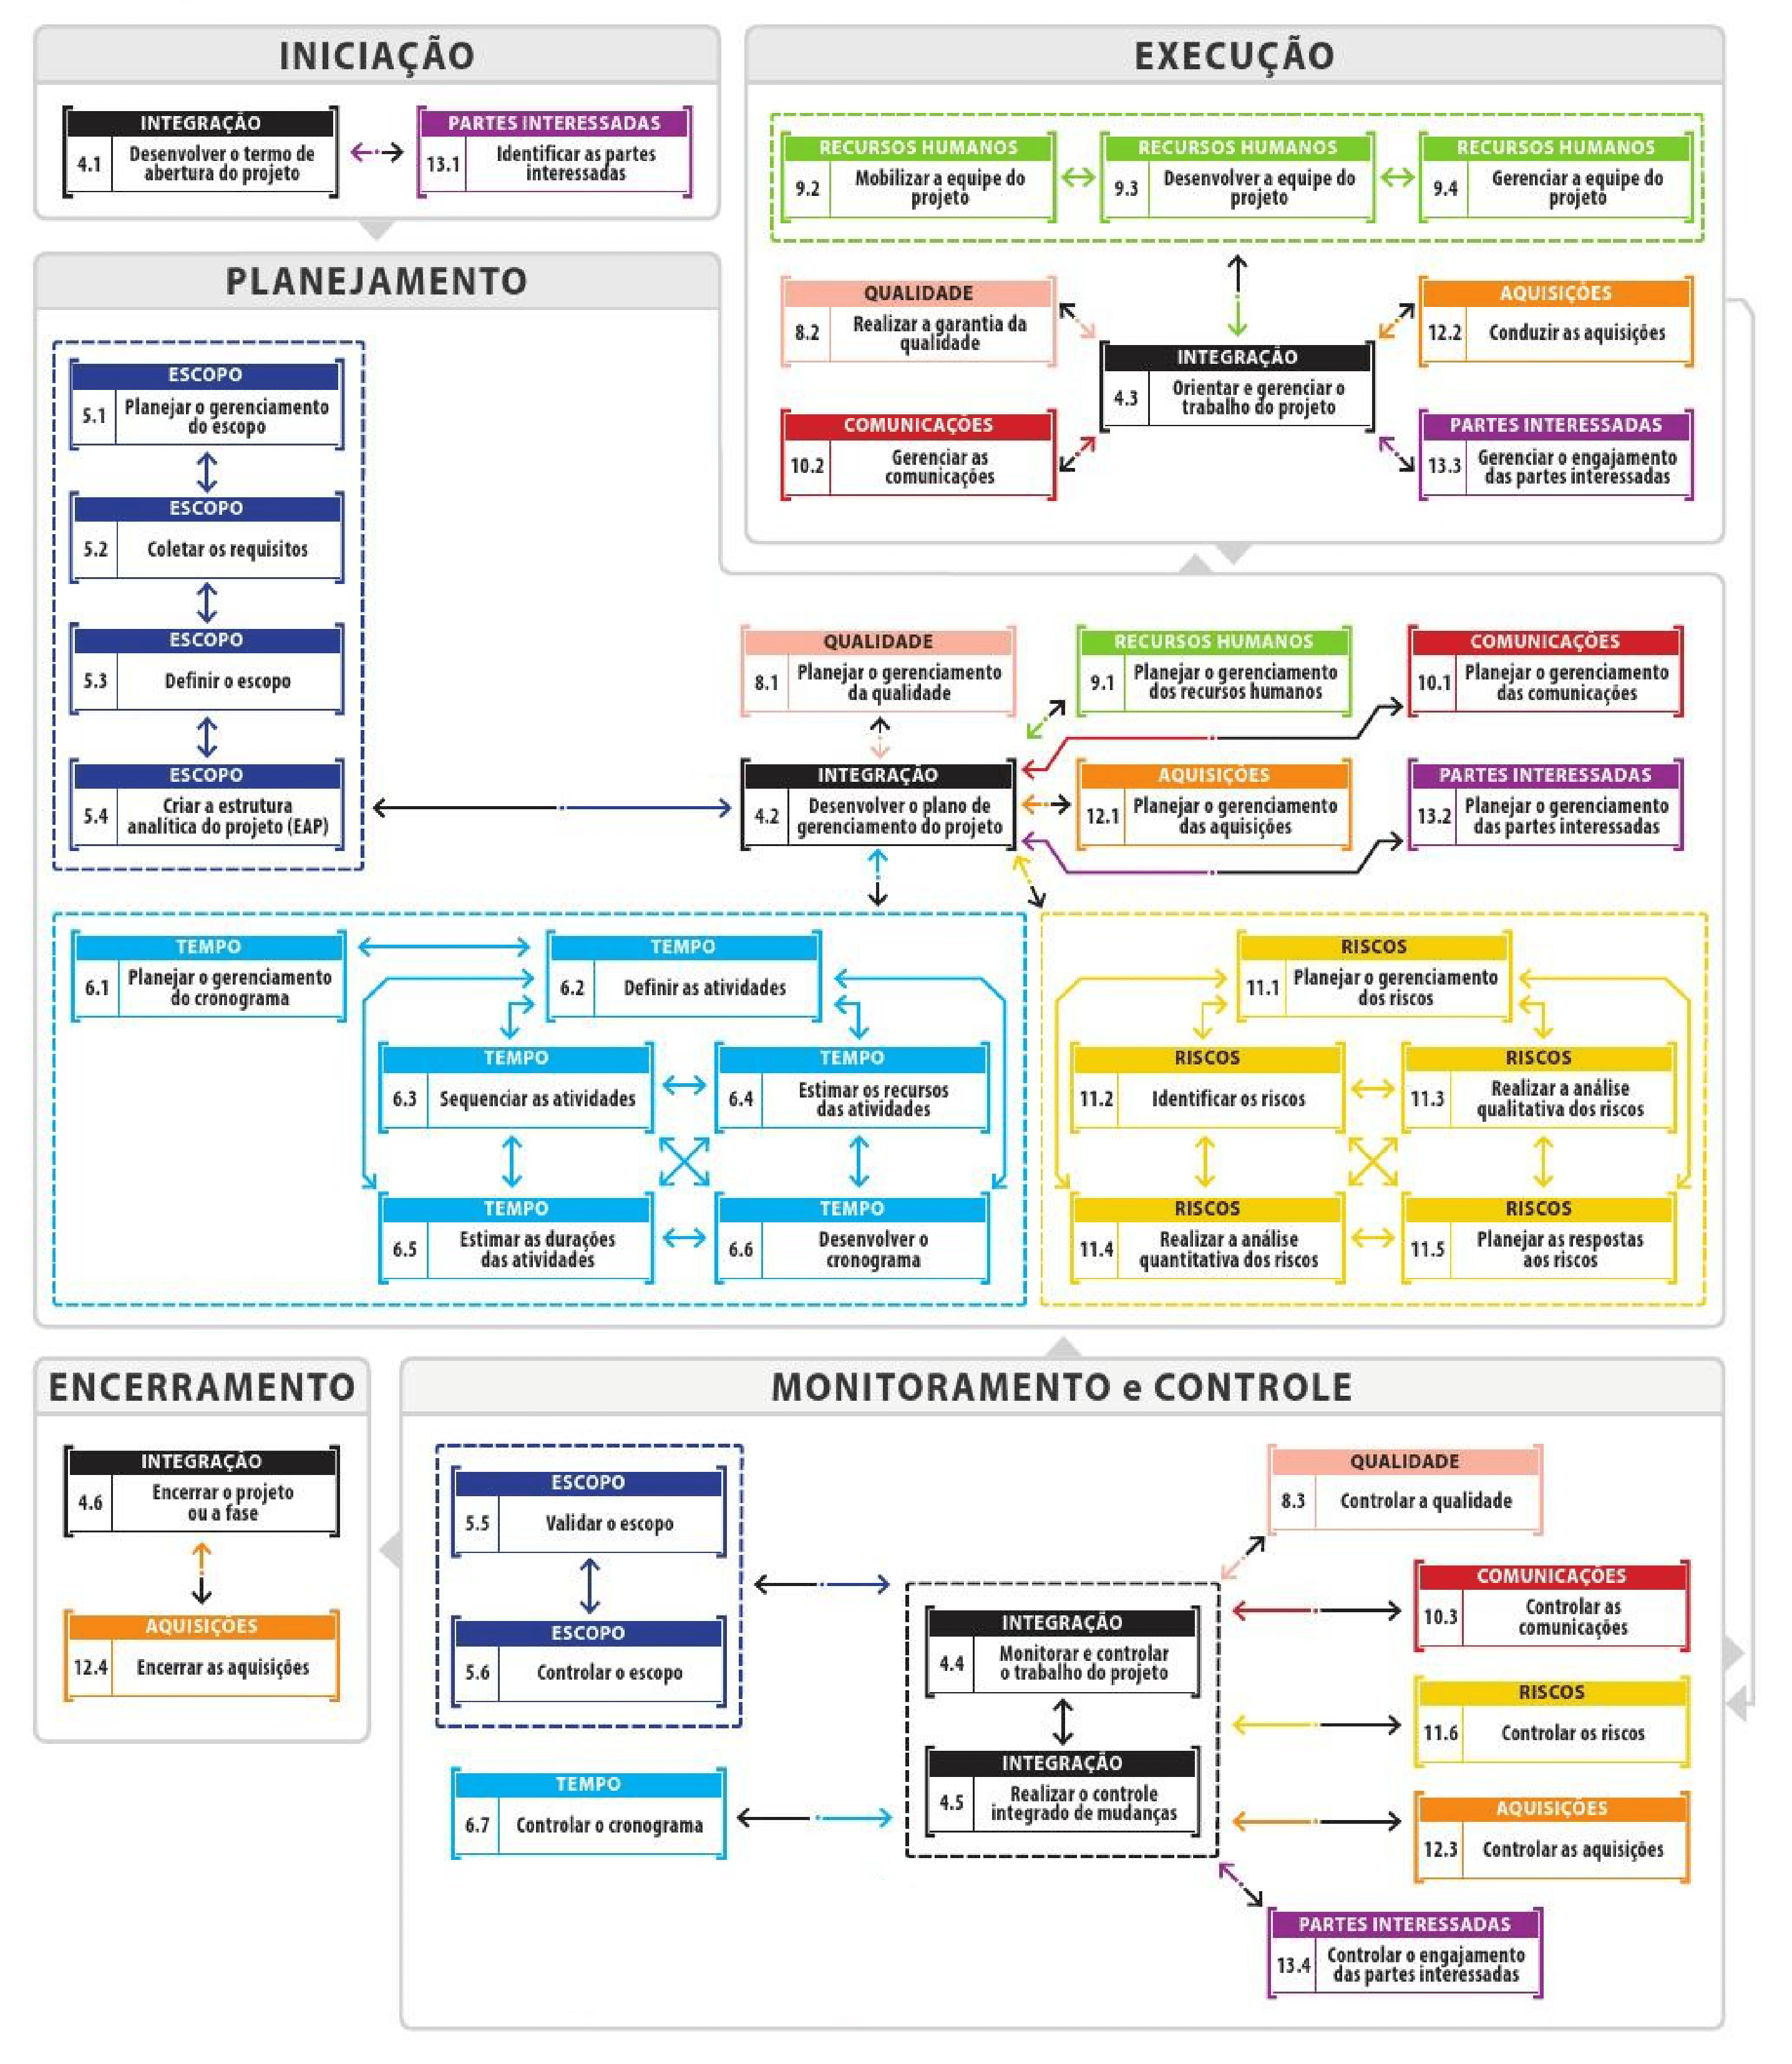
\includegraphics[scale=0.24]{./Figuras/fluxo-processos.png}
		\end{center}
		\legend{Fonte: os autores (2020)}
	\end{figure}
	
	
	
	{\textbf{Iniciação} - Esta é a fase inicial do projeto, nela é determinado a necessidade do projeto, com seus objetivos e justificativas, então é realizado os documentos iniciais onde as melhores estratégias são identificadas e selecionadas.}
	
	{\textbf{Planejamento} - Fase onde deve ser detalhado minuciosamente tudo aquilo que será realizado no projeto, desde cronogramas, interdependências entre atividades, alocação dos recursos envolvidos, análise de custos etc. Esta parte é muito importante pois a execução do projeto será em cima destas atividades para que sejam executadas sem dificuldades e imprevistos.}
	
	{\textbf{Execução} - Nesta fase tudo é onde tudo que foi planejado anteriormente se torne realidade, tendo que ser executado e realizado conforme planejado, qualquer erro cometidas nas fases anteriores fica evidente durante essa fase. }
	
	{\textbf{Monitoramento e Controle} - Esta fase acontece paralelamente às demais fases do projeto, acompanhando e controlando aquilo que está sendo realizado no projeto como um todo, podendo propor ações corretivas e preventivas no menor espaço de tempo possível após a detecção de erros.}


\section{Protótipo}

{\color{red} Reduzir o numero de imagens dessa section}

A prototipação é uma etapa de suma importância no desenvolvimento de projeto de software. Além de melhorar a produtividade da equipe, ela facilita o entendimento dos requisitos do sistema e permite a apresentação de de conceitos e funcionalidades da aplicação de modo simplificado.
Nesse trabalho foi utilizado a prototipação visual cujo ênfase se aplica a estética e usabilidade. Nesse tipo de protótipo é possível identificar o layout e a identidade visual da aplicação. \cite{dextra2013prototipacao}

{Protótipos podem ser gerados de acordo com as seguintes categorias \cite{coyette2004sketchixml}: protótipos em baixa fidelidade que focam na interação, em componentes de interface e na estrutura geral do sistema; protótipos em alta fidelidade que produzem uma imagem real do sistema; protótipos executáveis que produzem o código em uma linguagem de programação, focando em navegação, mas sem ainda levar em consideração as regras de negócio. Cada categoria serve para um propósito específico: protótipos em baixa fidelidade são úteis para demonstrar aos usuários quais atividades o sistema atende e as possibilidades de navegação no sistema, assim como para proporcionar uma visão geral do sistema. Protótipos em alta fidelidade são úteis para demonstrar padrões e guias de estilo. Protótipos executáveis são úteis para demonstrar navegação e testar o uso da interface \cite{rosemberg2008prototipaccao}.Seguindo as definições, o projeto desenvolvido utiliza os protótipos de baixa fidelidade}

\section{Aplicação WEB}
A aplicação web tem como foco o gerenciamento de toda a aplicação envolvendo consultas e cadastros gerais do sistema.
Apesar desse foco acentuado à gestão, é possível desempenhar todos os papeis dentro da aplicação web.


\subsection{Login}

\begin{figure}[htb]
	\caption{\label{web_login}Tela de Login do Agil.It}
	\begin{center}
		\includegraphics[scale=0.70]{./Figuras/web/login.png}
	\end{center}
	\legend{Fonte: os autores (2020)}
\end{figure}

A tela \ref{web_login} será a página responsável por autenticar os usuários e garantir a segurança do sistema.


\subsection{Cadastro de Ordem de Manutenção}

\begin{figure}[htb]
	\caption{\label{web_cad-om}Cadastro de Ordem de Manutenção}
	\begin{center}
		\includegraphics[scale=0.65]{./Figuras/web/cad-om.png}
	\end{center}
	\legend{Fonte: os autores (2020)}
\end{figure}

Na tela \ref{web_cad-om} é cadastrada e atualizada ordens de manutenção. Ela terá acesso às operações, componentes e assinaturas.


\subsection{Monitor de Ordem de Manutenção: Cards}

\begin{figure}[htb]
	\caption{\label{web_monitor-om-card}Monitor de Ordem de Manutenção: Cards}
	\begin{center}
		\includegraphics[scale=0.45]{./Figuras/web/monitor-om-card.png}
	\end{center}
	\legend{Fonte: os autores (2020)}
\end{figure}

A tela \ref{web_monitor-om-card} permite a consulta rápida e dinâmica das ordens de manutenção. Nela você pode aplicar os filtros de acordo com as \newline necessidades e será listada em forma de cartões, eles darão acesso à uma tela de detalhamento de ordem de manutenção.

\newpage
\subsection{Monitor de Ordem de Manutenção: Listas}

\begin{figure}[htb]
	\caption{\label{web_monitor-om-lista}Monitor de Ordem de Manutenção: Listas}
	\begin{center}
		\includegraphics[scale=0.45]{./Figuras/web/monitor-om-lista.png}
	\end{center}
	\legend{Fonte: os autores (2020)}
\end{figure}

A tela \ref{web_monitor-om-lista} permite a consulta rápida e dinâmica das ordens de manutenção. Nela você pode aplicar os filtros de acordo com as \newline necessidades e será listada em forma de listas, eles darão acesso à uma tela de detalhamento de ordem de manutenção.

\newpage
\subsection{Ordem de Manutenção}

\begin{figure}[htb]
	\caption{\label{web_om-capa}Ordem de Manutenção}
	\begin{center}
		\includegraphics[scale=0.40]{./Figuras/web/om-capa.png}
	\end{center}
	\legend{Fonte: os autores (2020)}
\end{figure}

Na tela \ref{web_om-capa} será possível acompanhar o andamento de uma ordem de manutenção de lista, ver informações referente à ordem e executar ações nela, como alterar status, adicionar operações e realizar assinaturas.

\newpage
\subsection{Checklist de Segurança}

\begin{figure}[htb]
	\caption{\label{web_check-list}Checklist de Segurança}
	\begin{center}
		\includegraphics[scale=0.40]{./Figuras/web/check-list.png}
	\end{center}
	\legend{Fonte: os autores (2020)}
\end{figure}

Na tela \ref{web_check-list} o manutentor irá marcar a lista de segurança antes de iniciar a ordem de manutenção.

\newpage
\subsection{Operações da Ordem de Manutenção}

\begin{figure}[htb]
	\caption{\label{web_om-operacoes}Operações da Ordem de Manutenção}
	\begin{center}
		\includegraphics[scale=0.40]{./Figuras/web/om-operacoes.png}
	\end{center}
	\legend{Fonte: os autores (2020)}
\end{figure}

Na tela \ref{web_om-operacoes} é possível verificar todas as operações pré cadastradas para a OM e cadastrar novas operações conforme necessidade para o andamento da OM.

\newpage
\subsection{Ordem de Manutenção: Lista}

\begin{figure}[htb]
	\caption{\label{web_om-lista}Ordem de Manutenção: Lista}
	\begin{center}
		\includegraphics[scale=0.40]{./Figuras/web/om-lista.png}
	\end{center}
	\legend{Fonte: os autores (2020)}
\end{figure}

Na tela \ref{web_om-lista} será possível acompanhar o andamento de uma ordem de manutenção de lista, ver informações referente à ordem e executar ações nela, como alterar status, adicionar operações e realizar assinaturas.

\newpage
\subsection{Equipamentos da Ordem de Manutenção: Lista}

\begin{figure}[htb]
	\caption{\label{web_om-lista-equipamentos}Equipamentos da Ordem de Manutenção: Lista}
	\begin{center}
		\includegraphics[scale=0.40]{./Figuras/web/om-lista-equipamentos.png}
	\end{center}
	\legend{Fonte: os autores (2020)}
\end{figure}

Na tela \ref{web_om-lista-equipamentos} será possível acompanhar os equipamentos que terão de ser inspecionados pelo manutentor e o mesmo marcar se executou ou não.

\newpage
\subsection{Ordem de Manutenção: Rota}

\begin{figure}[htb]
	\caption{\label{web_om-rota}Ordem de Manutenção: Rota}
	\begin{center}
		\includegraphics[scale=0.40]{./Figuras/web/om-rota.png}
	\end{center}
	\legend{Fonte: os autores (2020)}
\end{figure}

Na tela \ref{web_om-rota} será possível acompanhar o andamento de uma ordem de manutenção de lista, ver informações referente à ordem e executar ações nela, como alterar status, adicionar operações e realizar assinaturas.

\newpage
\subsection{Convidar ou Delegar Ordem de Manutenção}

\begin{figure}[htb]
	\caption{\label{web_om-convidar-delegar}Convidar ou Delegar Ordem de Manutenção}
	\begin{center}
		\includegraphics[scale=0.40]{./Figuras/web/om-convidar-delegar.png}
	\end{center}
	\legend{Fonte: os autores (2020)}
\end{figure}

Na tela \ref{web_om-convidar-delegar} será possível convidar técnicos para se juntarem a ordem de manutenção ou delegar a ordem de manutenção a outro manutentor. Ação só permitida àqueles que são responsáveis pela ordem de manutenção, ou seja, os que assumiram ela.

\newpage
\subsection{Apontamentos}

\begin{figure}[htb]
	\caption{\label{web_om-apontamentos}Apontamentos da Ordem de Manutenção}
	\begin{center}
		\includegraphics[scale=0.40]{./Figuras/web/om-apontamentos.png}
	\end{center}
	\legend{Fonte: os autores (2020)}
\end{figure}

Na tela \ref{web_om-apontamentos} será possível visualizar todos os apontamentos que existem em uma ordem, atualizá-las, excluí-las ou adicionar novos apontamentos.

\newpage
\subsection{Adicionar Apontamentos}

\begin{figure}[htb]
	\caption{\label{web_om-add-apontamento}Adicionar Apontamentos na Ordem de Manutenção}
	\begin{center}
		\includegraphics[scale=0.40]{./Figuras/web/om-add-apontamento.png}
	\end{center}
	\legend{Fonte: os autores (2020)}
\end{figure}

Na tela \ref{web_om-add-apontamento} será possível adicionar novos apontamentos a ordem de manutenção.

\newpage
\subsection{Motivo da Exclusão do Apontamento da Ordem de Manutenção}

\begin{figure}[htb]
	\caption{\label{web_om-excluir-apontamento-motivo}Motivo da Exclusão do Apontamento da Ordem de Manutenção}
	\begin{center}
		\includegraphics[scale=0.40]{./Figuras/web/om-excluir-apontamento-motivo.png}
	\end{center}
	\legend{Fonte: os autores (2020)}
\end{figure}

Na tela \ref{web_om-excluir-apontamento-motivo} o operador terá de informar o motivo pela exclusão do apontamento da ordem de manutenção.

\newpage
\subsection{Assinatura Digital}

\begin{figure}[htb]
	\caption{\label{web_om-assinatura}Assinatura Digital}
	\begin{center}
		\includegraphics[scale=0.40]{./Figuras/web/om-assinatura.png}
	\end{center}
	\legend{Fonte: os autores (2020)}
\end{figure}

Na tela \ref{web_om-assinatura} será possível assinar a ordem digitalmente. Para tanto, será cobrado as credenciais do operador.

\newpage
\section{Aplicação Mobile}
A aplicação Mobile é um ponto estratégico do produto, pois sua mobilidade permite com que os técnicos possam atuar na manutenção e realizar anotações e apontamentos no sistema através de um smartphone ou tablet.

\subsection{Login}

\begin{figure}[htb]
	\caption{\label{mobile_login}Login}
	\begin{center}
		\includegraphics[scale=0.80]{./Figuras/mobile/login.png}
	\end{center}
	\legend{Fonte: os autores (2020)}
\end{figure}

A tela \ref{mobile_login} será a página responsável por autenticar o usuário e garantir a segurança do sistema.

\newpage
\subsection{Menu}

\begin{figure}[htb]
	\caption{\label{mobile_menu}Menu}
	\begin{center}
		\includegraphics[scale=0.80]{./Figuras/mobile/menu.png}
	\end{center}
	\legend{Fonte: os autores (2020)}
\end{figure}

A figura \ref{mobile_menu} demonstra o menu lateral do aplicativo, identificando o usuário autenticado e um menu de acesso rápido às principais telas do sistema.

\newpage
\subsection{Monitor}

\begin{figure}[htb]
	\caption{\label{mobile_monitor}Monitor}
	\begin{center}
		\includegraphics[scale=0.75]{./Figuras/mobile/monitor.png}
	\end{center}
	\legend{Fonte: os autores (2020)}
\end{figure}

Na figura \ref{mobile_monitor} é possível verificar o monitor do manutentor. Nesse monitor, o manutentor consegue rapidamente visualizar as OMs pendentes e seus respectivos status através das bandeiras indicadas no card. As  vermelhas indicam que a OM tem uma prioridade emergente, as amarelas têm prioridade alta, as azuis têm prioridade média e as verdes possuem uma prioridade baixa.

\newpage
\subsection{Central de Notificações}

\begin{figure}[htb]
	\caption{\label{mobile_notificacao}Notificações}
	\begin{center}
		\includegraphics[scale=0.80]{./Figuras/mobile/notificacao.png}
	\end{center}
	\legend{Fonte: os autores (2020)}
\end{figure}

Na tela \ref{mobile_notificacao} é possível verificar notificações do usuário autenticado no sistema.

\newpage
\subsection{Ordem de Manutenção}

\begin{figure}[htb]
	\caption{\label{mobile_om}Ordem de Manutenção}
	\begin{center}
		\includegraphics[scale=0.70]{./Figuras/mobile/om.png}
	\end{center}
	\legend{Fonte: os autores (2020)}
\end{figure}

Na tela \ref{mobile_om} será possível acompanhar o andamento de uma ordem de manutenção preventiva e corretiva, ver informações referente à ordem e executar ações nela, como alterar status, adicionar operações e realizar assinaturas.

\newpage
\subsection{Ordem de Manutenção: Lista}

\begin{figure}[htb]
	\caption{\label{mobile_lista}Ordem de Manutenção: Lista}
	\begin{center}
		\includegraphics[scale=0.65]{./Figuras/mobile/lista.png}
	\end{center}
	\legend{Fonte: os autores (2020)}
\end{figure}

Na tela \ref{mobile_lista} será possível acompanhar o andamento de uma ordem de manutenção de lista, ver informações referente à ordem e executar ações nela, como alterar status, adicionar operações e realizar assinaturas.

\newpage
\subsection{Ordem de Manutenção: Rota}

\begin{figure}[htb]
	\caption{\label{mobile_rota}Ordem de Manutenção: Rota}
	\begin{center}
		\includegraphics[scale=0.70]{./Figuras/mobile/rota.png}
	\end{center}
	\legend{Fonte: os autores (2020)}
\end{figure}

Na tela \ref{mobile_rota} será possível acompanhar o andamento de uma ordem de manutenção de rota, ver informações referente à ordem e executar ações nela, como alterar status, adicionar operações e realizar assinaturas.

\newpage
\subsection{Checklist de Segurança}

\begin{figure}[htb]
	\caption{\label{mobile_checklist}Checklist de Segurança}
	\begin{center}
		\includegraphics[scale=0.80]{./Figuras/mobile/checklist.png}
	\end{center}
	\legend{Fonte: os autores (2020)}
\end{figure}

Na tela \ref{mobile_checklist} o manutentor irá marcar a lista de segurança antes de iniciar a ordem de manutenção.

\newpage
\subsection{Problemas}

\begin{figure}[htb]
	\caption{\label{mobile_problema}Problemas}
	\begin{center}
		\includegraphics[scale=0.80]{./Figuras/mobile/problemas.png}
	\end{center}
	\legend{Fonte: os autores (2020)}
\end{figure}

Na tela \ref{mobile_problema} o manutentor irá verificar com maiores detalhes os problemas identificados no equipamento.

\newpage
\subsection{Componentes}

\begin{figure}[htb]
	\caption{\label{mobile_componentes}Componentes da Ordem de Manutenção}
	\begin{center}
		\includegraphics[scale=0.70]{./Figuras/mobile/componentes.png}
	\end{center}
	\legend{Fonte: os autores (2020)}
\end{figure}

Na tela \ref{mobile_componentes} é possível verificar todos os componentes utilizados na operação da ordem de manutenção.

\newpage
\subsection{Operações}

\begin{figure}[htb]
	\caption{\label{mobile_operacao}Operações da Ordem de Manutenção}
	\begin{center}
		\includegraphics[scale=0.70]{./Figuras/mobile/operacao.png}
	\end{center}
	\legend{Fonte: os autores (2020)}
\end{figure}

Na tela \ref{mobile_operacao} é possível verificar todas as operações pré cadastradas para a OM e cadastrar novas operações conforme necessidade para o andamento da OM.

\newpage
\subsection{Apontamentos}

\begin{figure}[htb]
	\caption{\label{mobile_apontamentos}Apontamentos da Ordem de Manutenção}
	\begin{center}
		\includegraphics[scale=0.80]{./Figuras/mobile/apontamentos.png}
	\end{center}
	\legend{Fonte: os autores (2020)}
\end{figure}

Na tela \ref{mobile_apontamentos} é possível realizar os apontamentos das horas trabalhadas na execução da ordem de manutenção.

\newpage
\subsection{Assinatura Digital}

\begin{figure}[htb]
	\caption{\label{mobile_assinaturas}Assinatura Digital}
	\begin{center}
		\includegraphics[scale=0.80]{./Figuras/mobile/assinaturas.png}
	\end{center}
	\legend{Fonte: os autores (2020)}
\end{figure}

Na tela \ref{mobile_assinaturas} é possível verificar e realizar as assinaturas.
\chapter{Planejamento do Sistema}

O planejamento do sistema é crucial para o sucesso do projeto. Nele deve-se estipular cronogramas de desenvolvimento e fazer a análise de risco para calcular a probabilidade e impacto de problemas que possam ocorrer durante o desenvolvimento do projeto.
Um bom planejamento também deve ter uma análise de projeto que envolva recursos de diversas naturezas bem como humanos, capitais, técnicos e tecnológicos.
Outro ponto importante é a prototipação do sistema para ter uma avaliação inicial com os \textit{stakeholders} e ter uma base a ser seguida durante o desenvolvimento.

\section{Cronograma do Projeto}

Todo bom projeto deve ter um cronograma e um planejamento de ação, baseado nisso, foi elaborado dois cronogramas: um apresentando todo o conteúdo aprendido no semestre e outro montando plano de ação para implementação do projeto.

As figuras a seguir, são cronogramas que demonstram a trajetória do desenvolvimento do projeto. Divididos por semestre, os cronogramas listam as atividades aprendidas nas UCs, com todas as partes teóricas e práticas onde o objetivo principal é implementar todo conhecimento adquirido em prol de um projeto único: A unificação de todas as UCs do curso de Sistemas para Internet.

\begin{figure}[H]
\caption{\label{cron-3-semestre}Cronograma de Aprendizagem: Terceiro Semestre}
\begin{center}
	\includegraphics[scale=0.90]{./Figuras/cronograma-3-semestre.png}
\end{center}
\end{figure}


\begin{figure}[H]
\caption{\label{cron-4-semestre}Cronograma de Aprendizagem: Quarto Semestre}
\begin{center}
	\includegraphics[scale=0.90]{./Figuras/cronograma-4-semestre.png}
\end{center}
\end{figure}


\begin{figure}[H]
\caption{\label{cron-5-semestre}Cronograma de Aprendizagem: Quinto Semestre}
\begin{center}
	\includegraphics[scale=0.47]{./Figuras/cronograma-5-semestre.png}
\end{center}
\end{figure}

\begin{figure}[H]
	\caption{\label{cron-6-semestre}Cronograma de Aprendizagem: Sexto Semestre}
	\begin{center}
		\includegraphics[scale=0.52]{./Figuras/cronograma-6-semestre.png}
	\end{center}
\end{figure}

\section{Análise de riscos}

A análise de riscos tem como objetivo identificar os possíveis problemas durante e após o desenvolvimento do projeto a fim de elaborar um plano de ação para solucionar rapidamente o problema de fato \cite{schmitzanalise}.

Segundo \cite{de2003engenharia}, um grande volume de dados publicados aponta para os riscos que correm os projetos de software executados sem a utilização de processos adequados. Um levantamento publicado, a partir de
uma base de dados de 4.000 projetos, constatou a ocorrência frequente dos seguintes
problemas: 

\begin{itemize}
	
	\item 70\% dos projetos de grandes aplicativos sofre de instabilidade dos requisitos. Os requisitos crescem tipicamente cerca de 1\% ao mês, atingindo níveis de mais de 25\% de inchaço ao final
	do projeto.
	
	\item Pelo menos 50\% dos projetos são executados com níveis de produtividade abaixo do normal.
	
	\item Pelo menos 25\% do software de prateleira e 50\% dos produtos feitos por encomenda apresentam níveis de defeitos superiores ao razoável. 
	
	\item Produtos feitos sob pressão de prazos podem quadruplicar o número de defeitos.
	
	\item Pelo menos 50\% dos grandes projetos de software estouram seu orçamento e seu prazo.
	
\end{itemize}

Sendo assim, foi identificado os fatores de risco, no qual o projeto em questão possa estar exposto. Nela, faz-se uma análise do impacto e probabilidade de fatores prejudiciais ao projeto, conforme tabela \ref{tebela_risco} abaixo.

\begin{table}[h]
	\centering
	\caption{\label{tebela_risco} Tabela de Riscos Agil.it}
	\begin{tabular}{l|l|l}
		\hline
		\rowcolor[HTML]{EFEFEF} 
		\textbf{Riscos}                     & \textbf{Probabilidade} & \textbf{Impacto} \\ \hline
		\rowcolor[HTML]{DD7346} 
		Mudança de escopo                   & 90\%                   & 2                \\ \hline
		\rowcolor[HTML]{DD7346} 
		Entrega no prazo                    & 70\%                   & 3                \\ \hline
		\rowcolor[HTML]{DD7346} 
		Integração com SAP                  & 70\%                   & 2                \\ \hline
		\rowcolor[HTML]{FFFE65} 
		Implantação na empresa              & 60\%                   & 2                \\ \hline
		\rowcolor[HTML]{FFFE65} 
		Conexão com o banco de dados        & 60\%                   & 3                \\ \hline
		\rowcolor[HTML]{FFFE65} 
		Aceitação da usabilidade do sistema & 50\%                   & 2                \\ \hline
		\rowcolor[HTML]{FFFE65} 
		Usuários inexperientes              & 40\%                   & 2                \\ \hline
		\rowcolor[HTML]{9AFF99} 
		Mudanças na tecnologia              & 20\%                   & 3                \\ \hline
		\rowcolor[HTML]{9AFF99} 
		Segurança dos dados                 & 15\%                   & 2                \\ \hline
		\rowcolor[HTML]{9AFF99} 
		Conexão com a rede                  & 10\%                   & 2                \\ \hline
		\rowcolor[HTML]{9AFF99} 
		Falta de profissionais              & 5\%                    & 3                \\ \hline
	\end{tabular}
\end{table}

Na tabela \ref{tebela_risco} estão mapeados os principais riscos identificados para o projeto Agil.It. Nela, a probabilidade indica a chance do risco ocorrer, as cores acompanham a porcentagem da mesma, sendo 70\% ou mais a cor vermelha, entre 40\% e 69\% a cor amarela e de 0\% a 39\% a cor verde e o impacto é uma escala de um a três (1-3) do quanto o risco pode afetar a conclusão e entrega do projeto. A seguir será abordado o diagrama de causa e efeito.

{\subsection{Diagrama de Causa e Efeito}
	
	{\color{red} Descrever Diagrama de Causa e Efeito com referencias}
	
	
	\begin{figure}[htb]
		\caption{\label{causaeefeito1}Diagrama de Causa e Efeito}
		\begin{center}
			\includegraphics[scale=0.55]{./Figuras/Diagrama causa e efeito.jpeg}
		\end{center}
		\legend{Fonte: os autores (2020)}
	\end{figure}
}



\section{PMBOK}

{É uma metodologia de gerenciamento de projeto internacionalmente reconhecida, essas práticas podem auxiliar na resolução dos recursos humanos, capitais, tecnológicos e técnicos. Além disso, utilizando PMBOK é possível gerir melhor o andamento do projeto e de forma mais coordenada. Segundo \cite{PMG2018} o PMBOK tem conhecimentos já comprovados que são amplamente utilizados, assim como o conhecimento de práticas mais inovadoras e avançadas} Dentre as técnicas de planejamento, pode-se utilizar para estudos e desenvolvimento a EAP -  Estrutura Analítica de Projetos, descrita a seguir.

\subsection{Estrutura Analítica do Projeto}



{A Estrutura Analítica do Projeto (EAP) é a divisão estruturada de trabalho do projeto dividido em faixas gerenciadas cujo a sua totalidade significa em um entregável ao projeto final.
	
	Segundo \cite{PMI2018} o detalhamento da EAP deve chegar até o nível do pacote de trabalho, nível mais baixo na EAP, que é o ponto no qual o custo e o cronograma do trabalho podem ser estimados de forma confiável. Porém o nível de detalhamento desse pacote varia de acordo com a complexidade de cada projeto. \cite{kerzner2017} defende que a EAP deve ser composta por até três níveis pois se for detalhado com demaseio o custo com o gerenciamento serão também excessivos.}

Para o projeto Agil-it foi decidido utilizar 6 faixas de entregáveis:

\begin{subalineas}
	\item {Planejamento};
	\item {Análise};
	\item {Implementação Web};
	\item {Implementação Mobile};
	\item {Testes};
	\item {Implantação}.
\end{subalineas}


\begin{landscape}
	\begin{figure}[htb]
		\caption{\label{EAP}EAP AGIL.IT}
		\begin{center}
			\includegraphics[scale=0.38]{./Figuras/EAP.png}
		\end{center}
		\legend{Fonte: os autores (2020)}
	\end{figure}
\end{landscape}

A figura \ref{EAP} mostra a estrutura e o desenvolvimento que cada faixa requer no projeto. Ela não segue uma ordem cronológica, portanto não é necessário finalizar uma faixa para começar outra, muitas vezes elas são desenvolvidas em conjunto para uma melhor utilização do tempo de projeto.


\subsection{Fluxo de Processos}
% ---

{O fluxo de processo é subdividido em cinco fases principais sobre o fluxo do projeto, iniciação sendo a primeira seguindo de planejamento, execução, monitoramento, controle e finalização. Para \cite{PMG2018} um projeto é desenvolvido a partir de uma idéia, em seguida parte para um plano e após isso é executado e concluído.}

Para a definição dos processos, foi utilizado os seguintes recursos:

\begin{subalineas}
	\item {Partes Interessadas};
	\item {Escopo};
	\item {Tempo};
	\item {Recursos Humanos};
	\item {Aquisições};
	\item {Qualidade};
	\item {Comunicações};
	\item {Riscos}.
\end{subalineas}

A figura abaixo contém todos os fluxos desenhados para o projeto.

\begin{figure}[H]
	\caption{\label{Fluxo-Processos}Fluxo e Processos AGIL.IT}
	\begin{center}
		\includegraphics[scale=0.24]{./Figuras/fluxo-processos.png}
	\end{center}
	\legend{Fonte: os autores (2020)}
\end{figure}



{\textbf{Iniciação} - Esta é a fase inicial do projeto, nela é determinado a necessidade do projeto, com seus objetivos e justificativas, então é realizado os documentos iniciais onde as melhores estratégias são identificadas e selecionadas.}

{\textbf{Planejamento} - Fase onde deve ser detalhado minuciosamente tudo aquilo que será realizado no projeto, desde cronogramas, interdependências entre atividades, alocação dos recursos envolvidos, análise de custos etc. Esta parte é muito importante pois a execução do projeto será em cima destas atividades para que sejam executadas sem dificuldades e imprevistos.}

{\textbf{Execução} - Nesta fase tudo é onde tudo que foi planejado anteriormente se torne realidade, tendo que ser executado e realizado conforme planejado, qualquer erro cometidas nas fases anteriores fica evidente durante essa fase. }

{\textbf{Monitoramento e Controle} - Esta fase acontece paralelamente às demais fases do projeto, acompanhando e controlando aquilo que está sendo realizado no projeto como um todo, podendo propor ações corretivas e preventivas no menor espaço de tempo possível após a detecção de erros.}


\section{Protótipo}

A prototipação é uma etapa de suma importância no desenvolvimento de projeto de software. Além de melhorar a produtividade da equipe, ela facilita o entendimento dos requisitos do sistema e permite a apresentação de de conceitos e funcionalidades da aplicação de modo simplificado.
Nesse trabalho foi utilizado a prototipação visual cujo ênfase se aplica a estética e usabilidade. Nesse tipo de protótipo é possível identificar o layout e a identidade visual da aplicação. \cite{dextra2013prototipacao}

{Protótipos podem ser gerados de acordo com as seguintes categorias \cite{coyette2004sketchixml}: protótipos em baixa fidelidade que focam na interação, em componentes de interface e na estrutura geral do sistema; protótipos em alta fidelidade que produzem uma imagem real do sistema; protótipos executáveis que produzem o código em uma linguagem de programação, focando em navegação, mas sem ainda levar em consideração as regras de negócio. Cada categoria serve para um propósito específico: protótipos em baixa fidelidade são úteis para demonstrar aos usuários quais atividades o sistema atende e as possibilidades de navegação no sistema, assim como para proporcionar uma visão geral do sistema. Protótipos em alta fidelidade são úteis para demonstrar padrões e guias de estilo. Protótipos executáveis são úteis para demonstrar navegação e testar o uso da interface \cite{rosemberg2008prototipaccao}.Seguindo as definições, o projeto desenvolvido utiliza os protótipos de baixa fidelidade}

\section{Aplicação WEB}
A aplicação web tem como foco o gerenciamento de toda a aplicação envolvendo consultas e cadastros gerais do sistema.
Apesar desse foco acentuado à gestão, é possível desempenhar todos os papeis dentro da aplicação web.

\subsection{Cadastro de Usuário}

\begin{figure}[H]
	\caption{\label{web_cad-user}Cadastro de Usuários}
	\begin{center}
		\includegraphics[scale=0.70]{./Figuras/web/cad-user.png}
	\end{center}
	\legend{Fonte: os autores (2020)}
\end{figure}

A tela \ref{web_cad-user} é utilizada para cadastrar usuários no sistema. Caso queira atualizar um registro basta colocar o código dele no primeiro campo ou pesquisar no ícone de lupa. Para cadastrar um novo basta deixar o primeiro campo vazio.

\subsection{Monitor de Ordem de Manutenção: Cards}

\begin{figure}[H]
	\caption{\label{web_monitor-om-card}Monitor de Ordem de Manutenção: Cards}
	\begin{center}
		\includegraphics[scale=0.45]{./Figuras/web/monitor-om-card.png}
	\end{center}
	\legend{Fonte: os autores (2020)}
\end{figure}

A tela \ref{web_monitor-om-card} permite a consulta rápida e dinâmica das ordens de manutenção. Nela você pode aplicar os filtros de acordo com as necessidades e será listada em forma de cartões, eles darão acesso à uma tela de detalhamento de ordem de manutenção.

\subsection{Checklist de Segurança}

\begin{figure}[H]
	\caption{\label{web_check-list}Checklist de Segurança}
	\begin{center}
		\includegraphics[scale=0.45]{./Figuras/web/check-list.png}
	\end{center}
	\legend{Fonte: os autores (2020)}
\end{figure}

Na tela \ref{web_check-list} o manutentor irá marcar a lista de segurança antes de iniciar a ordem de manutenção. Essa listá será gerada dinamicamente de acordo com a parametrização de segurança cadastrado no sistema.

\section{Aplicação Mobile}
A aplicação Mobile é um ponto estratégico do produto, pois sua mobilidade permite com que os técnicos possam atuar na manutenção e realizar anotações e apontamentos no sistema através de um smartphone ou tablet.

\subsection{Monitor}

\begin{figure}[htb]
	\caption{\label{mobile_monitor}Monitor}
	\begin{center}
		\includegraphics[scale=0.75]{./Figuras/mobile/monitor.png}
	\end{center}
	\legend{Fonte: os autores (2020)}
\end{figure}

Na figura \ref{mobile_monitor} é possível verificar o monitor do manutentor. Nesse monitor, o manutentor consegue rapidamente visualizar as OMs pendentes e seus respectivos status através das bandeiras indicadas no card. As  vermelhas indicam que a OM tem uma prioridade emergente, as amarelas têm prioridade alta, as azuis têm prioridade média e as verdes possuem uma prioridade baixa.

\subsection{Central de Notificações}

\begin{figure}[H]
	\caption{\label{mobile_notificacao}Notificações}
	\begin{center}
		\includegraphics[scale=0.80]{./Figuras/mobile/notificacao.png}
	\end{center}
	\legend{Fonte: os autores (2020)}
\end{figure}

Na tela \ref{mobile_notificacao} é possível verificar notificações do usuário autenticado no sistema.

\subsection{Ordem de Manutenção}

\begin{figure}[H]
	\caption{\label{mobile_om}Ordem de Manutenção}
	\begin{center}
		\includegraphics[scale=0.70]{./Figuras/mobile/om.png}
	\end{center}
	\legend{Fonte: os autores (2020)}
\end{figure}

Na tela \ref{mobile_om} será possível acompanhar o andamento de uma ordem de manutenção preventiva e corretiva, ver informações referente à ordem e executar ações nela, como alterar status, adicionar operações e realizar assinaturas.
\chapter{Implementação}

Nessa etapa, o sistema codificado a partir da descrição computacional das fases de projeto, como visto nos capítulos anteriores, conta com três aplicações: WEB, Mobile e Servidor. As aplicações foram desenvolvidas ao longo de três semestres no qual disponibilizou-se períodos de implementação e apresentação aos envolvidos, sendo estes a Faculdade de Tecnologia Senai e a Indústria Duas Rodas com o objetivo de alinhar o desenvolvimento e as expectativas do software em relação ao processo de manutenção executado atualmente.

\section{Tecnologias}
Para o desenvolvimento do sistema, foram divididas em três aplicações: uma visando a parte WEB, outra visando dispositivos móveis com os sistemas Android e IOS e para efetuar a comunicação entre os sistemas e o banco dados, foi elaborado uma aplicação de servidor cujo valida as requisições e efetua a comunicação entre as aplicações visíveis e o banco de dados.

\subsection{Aplicação WEB}

Para o desenvolvimento foi utilizada as tecnologias pré requisitadas pela empresa Duas Rodas, sendo elas HTML5\footnote{\url{https://html.spec.whatwg.org/}}, SASS\footnote{\url{https://sass-lang.com/}} e como complemento, utilizamos a biblioteca ReactJS\footnote{\url{https://reactjs.org/}}.

{\textbf{HTML5} - É uma linguagem de marcação utilizada para desenvolvimento Web, esta nova versão traz consigo importantes mudanças quanto ao papel do HTML no mundo da Web, através de novas funcionalidades como semântica e acessibilidade.}

{\textbf{SASS} - É uma folha de estilo interpretada e compilada em Cascading style sheets, ao ser interpretado é criado blocos de códigos de regras CSS. Resumidamente é utilizada para fazer o Design do sistema, com cores personalizadas, etc.}

{\textbf{ReactJs} - O React é uma biblioteca JavaScript de código aberto com foco em criar interfaces de usuário em páginas web.}

\subsection{Aplicação Mobile}
Utilizando as tecnologias Ionic 4\footnote{\url{https://ionicframework.com/}} e TypeScript\footnote{\url{https://www.typescriptlang.org/}} esta aplicação é desenvolvida paralelamente com as demais aplicações, tem como objetivo a mobilidade, facilidade de acesso e interação podendo ser utilizado em qualquer lugar dentro da empresa.

{\textbf{TypeScript} - TypeScript é um superconjunto de JavaScript desenvolvido pela Microsoft que adiciona tipagem e alguns outros recursos a linguagem. É utilizada somente pelos desenvolvedores, pois auxilia na construção do código fonte. Seu código é transpilado para JavaScript, no final das contas tudo escrito em TypeScript vira JavaScript.}

{\textbf{Ionic 4} - O Ionic é um \textit{framework} de código aberto para desenvolvimento de aplicativos móveis multiplataforma.}

\subsection{Aplicação do Servidor}
A aplicação do servidor é o canal centralizador das demais plataformas. Ela tem acesso único e exclusivo ao banco de dados. É responsável por todas as validações e executa regras de negócio.
O servidor foi desenvolvido em Typescript e utiliza a TypeOrm\footnote{\url{https://typeorm.io/}} para integração com o banco de dados, para a API utiliza o Express\footnote{\url{https://expressjs.com/}}.

{\textbf{TypeOrm} - TypeOrm é uma ORM para Typescript, utiliza injeção de dependências para modelar as classes e transformar em tabelas.}

{\textbf{Express} - Express é uma biblioteca que abstrai a camada HTTP e gerencia requisições recebidas pelo protocolo.}


\section{Códigos Desenvolvidos} 

Nesta etapa será apresentado alguns trechos dos códigos implementados para ilustrar o funcionamento e o entendimento de partes específicas do código fonte, onde os mesmos contém regras complexas e de suma importância ao leitor.

\subsection{WEB}
\subsubsection{Componentes}
A plataforma web da Agil.It tem como padrão componentizar os elementos exibidos no \textit{front-end}, para isso, utiliza-se a biblioteca \textit{React-md}, com componentes acessíveis por propriedades (parâmetros) e totalmente personalizáveis. Os estilos podem ser configurados tanto em tempo de compilação quanto em tempo de execução pelas variáveis SASS configuráveis e pelo uso de CSS.
A biblioteca deve ser instalada no projeto e importada no código fonte conforme é mostrado no código \ref{react-md-components}.

\begin{lstlisting}[language=JavaScript, caption={Importando o componente de Ícone do react-md}, label={react-md-components}]
import React, { PureComponent } from 'react';
import { FontIcon } from 'react-md';

export class C_Icon extends React.Component {
	constructor(props) {
		super(props);
	}
	
	render() {
		return (
			<FontIcon 
				className={this.props.className}
				primary={this.props.primary}
				forceFontSize={!!this.props.iconSize}
				secondary={this.props.secondary}
				forceSize={this.props.iconSize}
				label={this.props.label}
				style={this.props.style}
				onClick={this.props.action}
				disabled={this.props.disabled}
				name={this.props.name}
			>
				{this.props.icon}
			</FontIcon>
		);
	}
}
\end{lstlisting}

\subsubsection{Cookies}
Ao efetuar o login na plataforma, as informações do usuário, exceto sua senha, são armazenadas nos \textit{cookies} através da biblioteca \textit{universal-cookie} e são manipuladas para ocultar telas de determinados usuários de acordo com o seu perfil ou exibir alguma tela adicional de controle e análise, caso o perfil logado seja de um administrador. Outro exemplo seria impedir/permitir que tal usuário possa executar determinada ação ocultando elementos na tela de acordo com seu perfil.
Com isso, o controle de informações e ações que o sistema oferece se torna muito mais fácil.

Após cada requisição feita ao servidor, o mesmo retorna um novo \textit{token} renovado e então atualiza-se o \textit{token} e usuário do \textit{cookie}.
Conforme demonstrado no código \ref{storage-cookie-data}

\begin{lstlisting}[language=JavaScript, caption={Gravar dados no cookie}, label={storage-cookie-data}]
setToken(token) {
	const user = JWTHelper.decomposeJwt(token)

	this.cookies.set('token', token, { path: '/' })
	this.cookies.set('user', user, { path: '/' })
}
\end{lstlisting}

Para recuperar os valores dos \textit{cookies} basta instanciar o \textit{universal-cookies} e utilizar o método \textit{get}. Para remover o dado basta utilizar o método \textit{remove}, de acordo com o código \ref{universal-cookie-methods}.

\begin{lstlisting}[language=JavaScript, caption={Recuperar dados do cookie}, label={universal-cookie-methods}]
class App extends Component {
	constructor() {
		super()

		this.cookies = new Cookies();

		this.state = { 
			token: this.cookies.get('token'),
			user: this.cookies.get('user'),
		};
	};
	
	onLogout() {
		this.cookies.remove('token');
		this.setState({ token: undefined })
	}
}
\end{lstlisting}

\subsubsection{Helpers}
Com o objetivo de agilizar o desenvolvimento do projeto, foram implementadas diversas classes de ajuda como \textit{DateHelper}, \textit{MaintenanceOrderHelpers} e \textit{SearchModel}.

\textit{DateHelper} é responsável por manipular e retornar as datas no formato desejado, possui funções que podem ser chamadas em qualquer classe para auxiliar o time de desenvolvimento no ganho de tempo. Como manipular datas é trabalhoso, segue um exemplo de como deixar um pouco mais simples, como pode-se ver no código \ref{date-helper}.

\begin{lstlisting}[language=JavaScript, caption={Função que formata a data em dia/mês/ano - horas/minutos}, label={date-helper}]
static formatDateTime(inputDate) {
	var date = this.getDate(inputDate);
	
	var day = StringHelper.JustifyLeft(date.getDate(), 2, 0);
	var month = StringHelper.JustifyLeft(date.getMonth() + 1, 2, 0);
	var year = date.getFullYear();
	var hour = date.getHours();
	var minutes = date.getMinutes();
	
	return `${day}/${month}/${year} às ${hour}h${minutes}`;
}
\end{lstlisting}

A \textit{MaintenanceOrderHelper} é responsável por auxiliar na manipulação dos dados referentes as ordens de manutenção, possui funções que fazem a tradução de algumas propriedades dos objetos que são salvos em inglês no servidor.

Código \ref{maintenance-order-helper-translate-props} exemplifica a utilização da função de tradução de propriedades da ordem na classe de Ordem de Manutenção.

\begin{lstlisting}[language=JavaScript, caption={Utilizando a tradução de propriedades da ordem de manutenção}, label={maintenance-order-helper-translate-props}]
<span>{HelperOM.translate("status", order.orderStatus)}</span>
<span>{HelperOM.translate("color", order.orderStatus)}</span>
<span>{HelperOM.translate("layout", order.orderLayout)}</span>
<span>{HelperOM.translate("priority", order.priority)}</span>
\end{lstlisting}

Código \ref{maintenance-order-helper-translate-method} demonstra a função que traduz as propriedades da Ordem.

\begin{lstlisting}[language=JavaScript, caption={Função de tradução}, label={maintenance-order-helper-translate-method}]
static translate(prop, value) {
	let props;
	
	if (prop == "priority") props = this.getPriority();
	else if (prop == "status") props = this.getStatus();
	else if (prop == "color") props = this.getColorPriority();
	else if (prop == "layout") props = this.getLayoutType();
	else return value;
	
	return props[value];
}

static getLayoutType() {
	return {
		default: 'Corretiva | Preventiva',
		route: 'ROTA',
		list: 'LISTA',
	}
}

static getColorPriority() {
	return {
		low: "#03a140",
		medium: "#3177e8",
		high: "#ffd300",
		urgent: "red",
	}
}

static getPriority() {
	return {
		low: "Baixa",
		medium: "Média",
		high: "Alta",
		urgent: "Urgente",
	}
}

static getStatus() {
	return {
		created: "Aberta",
		assumed: "Assumida",
		started: "Iniciada",
		paused: "Pausada",
		stopped: "Parada",
		canceled: "Cancelada",
		"signature-pending": "Assinatura Pendente",
		signatured: "Assinada",
		finished: "Finalizada",
		"no_status": "Sem Status",
	};
}
\end{lstlisting}

Ainda no \textit{MaintenanceOrderHelper} existem funções que ordenam as OM por prioridade e data de abertura na tela de monitoramento.
As ordens serão ordenadas das urgentes às com baixa prioridade e como um segundo fator será a data de abertura, sendo as mais antigas mostradas primeiro.

Código \ref{maintenance-order-helper-sort} mostra a lógica utilizada para a ordenação.

\begin{lstlisting}[language=JavaScript, caption={Funções responsáveis pela ordenação}, label={maintenance-order-helper-sort}]
static sortOrders(list) {
	var ordenatedPriority = this.ordenatedPriority();
	
	return list.sort((a, b) => {
		if (ordenatedPriority[a.priority] > ordenatedPriority[b.priority]) return -1;
		else if (ordenatedPriority[a.priority] < ordenatedPriority[b.priority]) return 1;
		
		var dateTimeA = DateHelper.getDate(a.openedDate).getTime();
		var dateTimeB = DateHelper.getDate(b.openedDate).getTime();
		
		if (dateTimeA > dateTimeB) return 1;
		else if (dateTimeA == dateTimeB) return 0;
		else return -1;
	});
}

static ordenatedPriority() {
	return {
		urgent: 3,
		high: 2,
		medium: 1,
		low: 0,
	};
}
\end{lstlisting}

O \textit{SearchModel} contém funções pré-configuradas das colunas que serão exibidas nas telas de CRUD afim de uma melhor visualização e organização dos dados exibidos.
A configuração é composta por um \textit{array} de objetos que possui três propriedades: \textit{name}, \textit{property} e \textit{defaultValue}.
A propriedade \textit{name} será o cabeçalho da coluna da tabela, \textit{property} é a propriedade da listagem que será renderizado na coluna e \textit{defaultValue} é o valor que será apresentado caso não haja dados para a \textit{property} na listagem.

Código \ref{search-model-data-config} mostra a definição da configuração do \textit{SearchModel}.

\begin{lstlisting}[language=JavaScript, caption={Definição da configuração para consulta de dados}, label={search-model-data-config}]
const machineTypeColumns = () => [
	{
		name: "ID",
		property:"id",
		defaultValue: "Sem ID",
	},
	{
		name: "Descrição",
		property:"description",
		defaultValue: "Sem Descrição",
	},
];

const equipmentColumns = () => [
	{
		name: "Código",
		property:"code",
		defaultValue: "Sem Código",
	},
	{
		name: "Descrição",
		property:"description",
		defaultValue: "Sem Descrição",
	},
	{
		name: "Tipo Máquina",
		property:"machineType.description",
		defaultValue: "Sem Tipo de Máquina",
	},
];
\end{lstlisting}

O código \ref{search-model-equipment} mostra a utilização das funções de busca na classe de cadastro de equipamentos.

\begin{lstlisting}[language=JavaScript, caption={Tela para cadastro de equipamento}, label={search-model-equipment}]
class CreateMachine extends Component {
	
	constructor(props) {
		super(props);
		
		this.state = {
			visible: true,
			equipmentId: '',
			machineType: '',
			fields: {},
			equipmentList: [],
			machineTypeList: [],
			equipmentColumns: equipmentColumns(),
			machineTypeColumns: machineTypeColumns(),
		};
	};
}
\end{lstlisting}

Ao obter as colunas em um \textit{state}, os dados são enviados ao componente \textit{C{\_}AutoComplete} que possui um ícone de lupa no qual o usuário pode clicar para visualizar todos os equipamentos cadastrados, conforme visto no código \ref{search-model-auto-complete}.

\begin{lstlisting}[language=JavaScript, caption={Utilizando o componente C\_AutoComplete}, label={search-model-auto-complete}]
	<C_AutoComplete
		id="id"
		name="id"
		value={this.state.equipmentId}
		label={"Equipamento"}
		rightIcon={"search"}
		list={this.state.equipmentList}
		searchColumns={this.state.equipmentColumns}
	/>
\end{lstlisting}

Código \ref{auto-complete-on-click-icon} mostra a função dentro do componente \textit{C{\_}AutoComplete} que exibe a tabela de consulta de acordo com as colunas e lista de dados enviados por parâmetro.

\begin{lstlisting}[language=JavaScript, caption={Componente C\_AutoComplete: Função executada ao clicar na lupa}, label={auto-complete-on-click-icon}]
	onClickIcon() {
		if (!Array.isArray(this.props.searchColumns)) return;
		
		confirmAlert({
			customUI: ({ onClose }) => (
				<C_SearchTable
					columns={this.props.searchColumns}
					content={this.props.list}
					onClick={this.tableSelected}
					extraFunction={onClose}
				/>
			)
		});
	}
\end{lstlisting}

\subsection{Mobile}
\subsubsection{Ações da Ordem de Manutenção}
A estrutura da classe \textit{AgilitActionUtils} é feita com o intuito de reutilizar códigos, sendo que cada tipo de OM deve ser assinada da mesma forma que qualquer outra, mudando apenas seu atributo identificador, a seguir seguem algumas características importantes desta classe.

A primeira característica desta classe é realizar as ações de uma determinada OM de forma centralizada, recebendo como parâmetro para qual OM deverá ser feita a ação e a ação propriamente dita, conforme mostra código \ref{order-actions}.

\begin{lstlisting}[language=JavaScript, caption={Alterar situação da ordem de manutenção}, label={order-actions}]
public async changeStatus(orderID, orderStatus : AgilitOrderStatus){    
	return this.restOrder.orderActions(orderID, orderStatus);
}

public orderActions(orderID : number, agilitOrderStatus : AgilitOrderStatus){
	const orderStatus : any = {
		orderStatus: agilitOrderStatus        
	}
	
	if (agilitOrderStatus == AgilitOrderStatus.ASSUMED){
		let userInfo : any = AgilitStorageUtils.getDataJSON(AgilitStorageTypes.USERDATA);
		
		orderStatus.userId = userInfo.id;
	}    
	
	this.http.url = this.http.getBaseUrl() + this.restAction + '/' + orderID + '/status';
	return ProviderHelper.put(this.http, orderStatus);
}

\end{lstlisting}

Outra característica muito importante desta classe é realizar as assinaturas de uma determinada OM, sendo passada como parâmetro a OM respectivamente e a senha de assinatura. Ao realizar uma assinatura a classe irá executar algumas validações da OM a fim de verificar se está de acordo para enviar ao servidor, com isso a promessa deve ser resolvida ou rejeitada.
O código \ref{sign-order-mobile} demonstra a implementação.

\begin{lstlisting}[language=JavaScript, caption={Assinar a ordem de manutenção}, label={sign-order-mobile}]
public async signOrder(order, assignaturePassword): Promise<any>{
	return new Promise(async (resolve, reject) => {
		this.resolvePromise = resolve;
		this.rejectPromise  = reject;
		
		try {
			if (!this.validateOrder(order, assignaturePassword)){
				return;
			}        
			
			const user = AgilitStorageUtils.getDataJSON(AgilitStorageTypes.USERDATA);
			
			if (AgilitUtils.isNullOrUndefined(user) || AgilitUtils.isNullOrUndefined(user.id) || user.id == ''){
				this.rejectPromise('Dados de usuário inválido!');
				return;
			}
			
			await this.restOrder.orderAssignature(order.id, user.id).then(
			(response: any) => {
				if (AgilitUtils.isNullOrUndefined(response)){
					return;
				}
				
				this.resolvePromise(response);
			}
			).catch(
			error => {
				this.rejectPromise(error);
			}
			);
		} catch (error) {
			this.rejectPromise(error);
		}
	});
}
\end{lstlisting}

Para que uma OM seja assinada com sucesso a classe deve conter as validações dos estados atuais da OM a ser assinada, por exemplo, se o usuário realizar a assinatura de uma OM com status cancelada esta implementação tem de validar a mesma.
Código \ref{order-validation} mostra a implementação de validação da ordem antes da assinatura.

\begin{lstlisting}[language=JavaScript, caption={Validar estados da OM}, label={order-validation}]
private validateOrder(order, password) : boolean{
	if (password != AgilitStorageUtils.getData(AgilitStorageTypes.PASSWORD)){
		this.rejectPromise('Senha incorreta!');
		return;
	}
	
	if (order.orderStatus == AgilitOrderStatus.SIGNATURED){
		this.rejectPromise('OM já está assinada!');
		return;
	}
	
	if (order.orderStatus == AgilitOrderStatus.FINISHED){
		this.rejectPromise('OM já está assinada!');
		return;
	}
	
	if (order.orderStatus == AgilitOrderStatus.CANCELED){      
		this.rejectPromise('OM está cancelada!');
		return;
	}
	
	return true;
}
\end{lstlisting}

\subsubsection{Dados Armazenados no Local Storage}
Algumas informações, por exemplo, usuário e token de acesso devem ficar salvas em memória para posteriormente serem utilizadas novamente, com isso desenvolvemos a classe chamada \textit{AgilitStorageUtils} contendo regras, limpezas específicas dos dados e separação dos tipos de dados que estão sendo armazenados e buscados.

O código \ref{AgilitStorageTypes} mostra os tipos de dados armazenados.
\begin{lstlisting}[language=JavaScript, caption={Tipos de dados armazenados}, label={AgilitStorageTypes}]
export enum AgilitStorageTypes{
	USERDATA = 'user',
	USERNAME = 'username',
	PASSWORD = 'password',
	TOKEN    = 'token'
}
\end{lstlisting}

O código \ref{AgilitStorageTypes-actions} mostra as ações de limpeza, busca e gravação de dados.

\begin{lstlisting}[language=JavaScript, caption={Tipos de dados armazenados}, label={AgilitStorageTypes-actions}]

// Remove de dados conforme o tipo especificado.
public static clearSpecificData(agilitStorageType : AgilitStorageTypes) {
	window.localStorage.removeItem(agilitStorageType);
}

// Buscando dados de um tipo específico armazenado na memória do navegador.
public static getData(agilitStorageType : AgilitStorageTypes) {
	return window.localStorage.getItem(agilitStorageType);
}

// Buscando dados de um tipo específico armazenado e convertendo para objeto.
public static getDataJSON(agilitStorageType : AgilitStorageTypes) {
	return JSON.parse(window.localStorage.getItem(agilitStorageType));
}

// Este método faz uma verificação do tipo do dado que está sendo inserido na memória do navegador.
public static setData(agilitStorageType : AgilitStorageTypes, data : Object|Array<any>|string) {
	if (AgilitUtils.isNullOrUndefined(data)){
		return;
	}
	
	if (typeof data === 'object'){
		window.localStorage.setItem(agilitStorageType, JSON.stringify(data));
		return;
	}
	
	if (typeof data === 'string'){
		window.localStorage.setItem(agilitStorageType, data);
	}    
}
\end{lstlisting}

\subsection{Servidor}
\subsubsection{Mapeamento do Banco de Dados com \textit{TypeOrm}}

A \textit{TypeOrm} trabalha com injeção de dependências, então em cada propriedade tem um \textit{decorator} que vai definir o mapeamento dela. Para gerar uma \textit{primary key} com auto increment, basta usar a injeção \textit{PrimaryGeneratedColumn}, para uma coluna simples, apenas \textit{column}, para data de criação do registro, \textit{CreateDateColumn} e para data de atualização do registro \textit{UpdateDateColumn}.
Com a \textit{TypeOrm} é possível ter classes abstratas para abranger propriedades em comum no banco de dados, para tanto foi criado a classe \textit{baseClass} que irá conter todos os campos em comum de todas as tabelas do banco de dados, conforme mostrado no código \ref{typeorm-base-class}.

\begin{lstlisting}[language=JavaScript, caption={BaseClass: Mapeamento de propriedades de tabelas do banco de dados}, label={typeorm-base-class}]
export abstract class BaseClass {
	
	@PrimaryGeneratedColumn()
	public id: number | undefined = undefined;
	
	@Column({ default: '' })
	public integrationID: string = '';
	
	@CreateDateColumn()
	public createdAt: Date | undefined = undefined;
	
	@Column()
	public createdBy: number | undefined = undefined;
	
	@UpdateDateColumn()
	public updatedAt: Date | undefined = undefined;
	
	@Column()
	public updatedBy: number | undefined = undefined;
	
	@Column({
		type: Boolean,
		default: false
	})
	public deleted: boolean = false;
	
	constructor() {
	}
	
}
\end{lstlisting}

Para facilitar as tabelas genéricas de CRUD, onde têm apenas os dados base e o campo de descrição, foi criado a classe abstrata \textit{crudClass}, conforme mostrado no código \ref{typeorm-crud-class}.

\begin{lstlisting}[language=JavaScript, caption={CrudClass: Mapeamento de propriedades para CRUDs genéricos}, label={typeorm-crud-class}]
export abstract class CrudClass extends BaseClass {

	@Column({nullable: false})
	@IsNotEmpty({
		message:'Descrição: Campo obrigatório.'
	})
	public description: string = '';

	constructor() {
		super();
	}
}
\end{lstlisting}

E por fim, o código \ref{model-sector} mostra a aplicação de uma classe que irá gerar de fato uma tabela no banco de dados.

\begin{lstlisting}[language=JavaScript, caption={Mapeamento de propriedades da tabela sector}, label={model-sector}]
@Entity('sector')
export class Sector extends CrudClass {

	constructor(){
		super();
	}

}
\end{lstlisting}

No primeiro parâmetro da injeção \textit{Entity} define-se o nome da tabela, e como a classe \textit{Sector} estende a classe \textit{CrudClass} que estende, subsequentemente a classe \textit{BaseClass} a tabela terá todas as colunas definidas nas injeções de dependências mostradas anteriormente.

Para fazer relações entre as tabelas existem alguns \textit{decorators} específicos: \textit{ManyToOne} para relações muitos para um, \textit{ManyToMany} para relações muitos para muitos, \textit{OneToOne} para relações um para um e \textit{OneToMany} para relações um para muitos.

O código \ref{model-installation-area} mostra a definição da relação \textit{ManyToOne}.

\begin{lstlisting}[language=JavaScript, caption={Mapeamento de propriedades da tabela área de installation\_area}, label={model-installation-area}]
@Entity("installation_area")
export class InstallationArea extends CrudClass {
	
	@ManyToOne(type => Sector, sector => sector.id, { nullable: false })
	@JoinColumn()
	public sector: Sector = undefined;
	
	constructor() {
		super();
	}
	
}
\end{lstlisting}

A \textit{TypeOrm} tenta fazer a relação automaticamente pelo nome dos campos, porém, se for uma relação mais complexa é possível usar o \textit{decorator JoinColumn} para definir qual coluna da tabela A se relaciona com qual coluna da tabela B e explicitar em qual das tabelas deve ficar a \textit{foreign key}, conforme mostrado no código \ref{model-maintenance-worker}.

\begin{lstlisting}[language=JavaScript, caption={Mapeamento de propriedades da tabela maintenance\_worker}, label={model-maintenance-worker}]
@Entity('maintenance_worker')
export class MaintenanceWorker extends BaseClass {

	@ManyToOne(type => User, user => user.id)
	@JoinColumn()
	public user : User;

	@ManyToOne(type => MaintenanceOrder, maintenanceOrder => maintenanceOrder.id, { cascade: false })
	@JoinColumn()
	public maintenanceOrder : MaintenanceOrder | undefined = undefined;

	@Column()
	public isMain: boolean = false;

	@Column()
	public isActive: boolean = false;

	@OneToMany(type => WorkerRequest, workerRequest => workerRequest.maintenanceWorker, { cascade: false })
	public workerRequest: Array<WorkerRequest>;

	@OneToMany(type => WorkedTime, workedTime => workedTime.maintenanceWorker, { cascade: false })
	public workedTime: Array<WorkedTime>;
}
\end{lstlisting}

\subsubsection{Validação de Objetos com o Class Validator}

Para validações de campos da tabela utiliza-se outra biblioteca com injeção de dependências que funciona muito bem quando mesclada com a \textit{TypeOrm}, o \textit{Class Validator}.
Com ele pode-se utilizar, por exemplo o \textit{decorator IsNotEmpty} na propriedade \textit{description}. Esse \textit{decorator} irá validar se a propriedade está vazia ou não, caso esteja, irá retornar o erro \textit{Descrição: Campo obrigatório.} conforme definição no próprio \textit{decorator} visto no código \ref{class-validator-model}.

\begin{lstlisting}[language=JavaScript, caption={Definição de validação de propriedades com o Class Validator}, label={class-validator-model}]
@IsNotEmpty({
message:'Descrição: Campo Obrigatório.',
})
public description: string = '';
\end{lstlisting}

E para executar a validação conforme as injeções feitas, é preciso importar a função \textit{validate} do \textit{class validator} e executar passando uma instancia do objeto.

\begin{lstlisting}[language=JavaScript, caption={Validação de Objetos com o Class Validator}]
async validate(entity: Entity) : Promise<any> {
	const errors = await validate(entity);
	
	if (errors.length === 0) {
		return undefined;
	}
	
	let errorList = [];
	
	errors.forEach(error => {
		let constraints = error.constraints;
		
		for (const key in constraints) {
			if (constraints.hasOwnProperty(key)) {
				errorList.push(constraints[key]);
			}
		}
	});
	
	return errorList;
}
\end{lstlisting}

O retorno vem em forma de \textit{array} e traz diversas informações a respeito dos erros ocorridos, no caso da API, é mostrado apenas a mensagem de erro em si, então a listagem é filtrada para mostrar apenas os erros.

\subsubsection{API}
Na API é utilizado o \textit{Express} para gerenciar as requisições feitas pela aplicação web, mobile e integração de sistemas externos.
Foi adicionado os \textit{plugins Cors} para lidar com o CORS, \textit{BodyParser} para converter JSON e o \textit{Helmet} para melhorar a segurança da aplicação.

No script de inicialização do servidor é estabelecido conexão com o banco de dados, instanciado a aplicação \textit{Express} e instalado seus \textit{plugins}, conforme visto no código \ref{script-inicial-servidor}

\begin{lstlisting}[language=JavaScript, caption={Script de inicialização do servidor}, label={script-inicial-servidor}]
createConnection().then(async connection => {

	// create express app
	const app = express();
	app.use(bodyParser.json());
	app.use(cors({exposedHeaders: 'token'}));
	app.use(helmet());

	// Get all system routes
	let routes = new Routes();

	routes.getCollections().forEach((collection: Collection) => {
		collection.getRoutes().forEach((route: Route) => {
			// Register each route
			route.registerRoute(app)
		});
	})

	
	app.listen(4000);

}).catch(error => console.log(error));
\end{lstlisting}

O roteamento é composto por várias coleções de rotas, no qual cada coleção tem um conjunto de rotas que é composto pela url que a rota responderá, os métodos que aceitará e a função que será invocada.
Por fim, o método \textit{registerRoute} irá registrar a rota da coleção ao \textit{express}.
Esses métodos que as rotas respondem ficam no \textit{package controller} que fazem a ponta entre receber a requisição, processar os dados recebidos e responder o que foi solicitado, seja cadastrar, atualizar, excluir ou consultar um ou mais registros.
Da mesma forma que foi feita com os \textit{models}, foi desenvolvido \textit{CrudController}, uma classe que utiliza \textit{Generics} que para cada instancia recebe o valor da entidade do CRUD e irá se adequar conforme o tipo fornecido. Essa classe também recebe no construtor o acesso ao repositório que será gravado, no caso, a tabela do banco de dados, conforme visto no código\ref{crud-controller}.

\begin{lstlisting}[language=JavaScript, caption={CrudController}, label={crud-controller}]
export class CrudController<Entity> {

	private repositoryEntity : Repository<Entity>;

	constructor(repositoryEntity: Repository<Entity>) {
		this.repositoryEntity = repositoryEntity;
	}
\end{lstlisting}

Todas as rotas são protegidas, com exceção da rota de login. Essa proteção é feita através de um \textit{middleware} colocado ao registrar a rota no \textit{express}, esse \textit{middleware} vai capturar os cabeçalhos \textit{token} para autenticação de sessão e \textit{authorization} para usuários de integração, caso nenhum dos cabeçalhos seja fornecido a API irá retornar o status ``401 - Unauthorized''. Caso seja passado o cabeçalho \textit{authorization} o \textit{middleware} irá verificar se chave informada é válida e se está na base de dados de usuários de integração. Se passado \textit{token}, o sistema irá decompor e validar o \textit{token} utilizando a biblioteca \textit{jsonwebtoken}, caso a validação do \textit{JWT} informado falhe, seja por não estar com a assinatura válida da aplicação ou por ter expirado o tempo da utilização, retorna um erro para a API informando que o \textit{token} não é válido. Caso a validação passe, o \textit{token} é regerado com expiração renovada para 5 horas e é adicionado ao cabeçalho da resposta. Lembrando que, o \textit{token} pode ser obtido pela primeira vez através da rota de Login.

O código \ref{middleware-check-jwt} demonstra a validação de usuário e \textit{token} feita pelo \textit{middleware} da API.
\begin{lstlisting}[language=JavaScript, caption={Função para validação de autenticação da API}, label={middleware-check-jwt}]
export const checkJwt = (request: Request, response: Response, next: NextFunction) => {
	
	const authorization = <string>request.headers["authorization"];
	
	if (authorization) {    // The Authorization was passed in so now we validate it
		this.checkIntegration(authorization)
		.then(valid => {
			if (valid === true) {
				return next();
			} else {
				return response.status(401).send();  
			}
		}).catch(err => {
			return response.status(500).send({
				"success": false,
				"error": err.message
			});
		})
	} else {
		//Get the jwt token from the request's header
		const token = <string>request.headers["token"];
		let jwtPayload;
		
		//Try to validate the token and get data
		try {
			jwtPayload = <any>jwt.verify(token, JWT.jwtSecret);
			response.locals.jwtPayload = jwtPayload;
		} catch (error) {
			//If token is not valid, respond with unauthorized
			return response.status(401).send();
		}
		
		//set to response's header the new token
		response.append('token', new UserController().generateJwtToken(<User> jwtPayload));
		
		//Call the next middleware or controller
		next();
	}
};

\end{lstlisting}


\subsubsection{Estratégia de Exclusão de Dados}

A estratégia para exclusão de dados adotado no projeto é não deletar os registros, mas alterar a coluna \textit{deleted} para \textit{true}. Desta maneira é possível rapidamente desfazer uma exclusão errada e também não ocorrerá problemas com histórico caso as entidades sejam deletadas.

Código \ref{remove-entity} mostra lógica executada durante a ``exclusão'' de um registro.
\begin{lstlisting}[language=JavaScript, caption={Método para exclusão de registro}, label={remove-entity}]
async removeEntity(entity: Entity) {
	entity["deleted"] = true;
	
	return this.getRepositoryEntity().save(entity)
}
\end{lstlisting}


\chapter{Agil.It}

No capítulo anterior foi detalhado as principais características da estrutura e organização do código fonte do sistema.
A seguir será apresentado as principais telas e funcionalidades disponíveis aos usuários.

\section{WEB}
A aplicação WEB tem seu foco na parte administrativa e gerencial do sistema, através dela o administrador poderá realizar os cadastros, assinaturas e acompanhar as situações de todas as ordens que estão em andamento.
\subsection{Cadastros do sistema}

\begin{figure}[H]
	\caption{\label{web-cadastros}Cadastros do Sistema}
	\begin{center}
		\includegraphics[scale=0.40]{./Figuras/agil.it/web-cadastros.png}
	\end{center}
	\legend{Fonte: os autores (2020)}
\end{figure}

A figura \ref{web-cadastros} mostra a lista de cadastros disponíveis no sistema.

\begin{figure}[H]
	\caption{\label{web-cadastro-equipamento}Cadastro de Equipamento}
	\begin{center}
		\includegraphics[scale=0.40]{./Figuras/agil.it/web-cadastro-equipamento.png}
	\end{center}
	\legend{Fonte: os autores (2020)}
\end{figure}

A figura \ref{web-cadastro-equipamento} mostra o cadastro de Equipamento, as demais telas de cadastro do sistema seguem o mesmo padrão, nas cores vermelho e branco e com campos de auto preenchimento conforme as informações são digitadas, os usuários conseguem efetuar a busca de dados de uma forma fácil e ágil. Os cadastros possuem também uma tela de consulta que fica visível ao clicar no ícone de lupa disponível no lado direito dos campos de auto preenchimento.
Entretanto, a tela Cadastro de Ordem de Manutenção é a única que contém abas para facilitar no preenchimento das informações por ser um cadastro mais extenso e trabalhoso.

Na figura \ref{web-search-table} mostra um exemplo de como fica a visualização da tela de consulta no cadastro de Equipamentos.

\begin{figure}[H]
	\caption{\label{web-search-table}Consulta de Equipamento}
	\begin{center}
		\includegraphics[scale=0.50]{./Figuras/agil.it/web-search-table.png}
	\end{center}
	\legend{Fonte: os autores (2020)}
\end{figure}

\subsection{Dashboard}

Essa tela tem como objetivo facilitar o monitoramento das ordens de manutenção, com a disponibilidade de filtros por data, status e prioridade os usuários conseguem encontrar o que desejam de uma forma muito mais rápida. Além disso, a Dashboard conta com duas opções de visualização das ordens listadas em tela, a primeira opção seria em forma de tabela com um filtro adicional por texto, conforme figura \ref{web-monitor-lista} e a segunda em forma de cards que contém cores para identificar a prioridade das ordens, conforme figura \ref{web-monitor-cards}.

\begin{figure}[H]
	\caption{\label{web-monitor-lista}Dashboard: Visualização por tabela}
	\begin{center}
		\includegraphics[scale=0.34]{./Figuras/agil.it/web-monitor-lista.png}
	\end{center}
	\legend{Fonte: os autores (2020)}
\end{figure}

\begin{figure}[H]
	\caption{\label{web-monitor-cards}Dashboard: Visualização por cards}
	\begin{center}
		\includegraphics[scale=0.34]{./Figuras/agil.it/web-monitor-cards.png}
	\end{center}
	\legend{Fonte: os autores (2020)}
\end{figure}

\subsection{Análise de Pendências de Assinatura}

\begin{figure}[H]
	\caption{\label{web-pendencias}Análise de pendências de assinatura}
	\begin{center}
		\includegraphics[scale=0.34]{./Figuras/agil.it/web-pendencias.png}
	\end{center}
	\legend{Fonte: os autores (2020)}
\end{figure}

A figura \ref{web-pendencias} mostra a tela de análise de pendências de assinatura que busca de forma automática todas as ordens de manutenção que estão com assinaturas pendentes seja pelo técnico, solicitante ou administrador. Os responsáveis pela ordem que ainda não assinaram são identificados pelo círculo na cor vermelha e os que já assinaram na cor verde. A ordem de manutenção irá permanecer na lista de pendências até ser exportada ao sistema SAP.
Apenas o usuário com o perfil administrador tem acesso a essa tela.

\subsection{Ordem de Manutenção}

\begin{figure}[H]
	\caption{\label{web-om}Ordem de Manutenção}
	\begin{center}
		\includegraphics[scale=0.34]{./Figuras/agil.it/web-om.png}
	\end{center}
	\legend{Fonte: os autores (2020)}
\end{figure}

Na figura \ref{web-om} é possível visualizar todas as informações relacionadas a ordem e todas as ações executadas nela, como por exemplo, quem solicitou a abertura de determinada ordem, a data e hora de abertura, todos os equipamentos e operações realizadas em cada um deles. Além disso, no canto superior direito da tela existe um menu com uma série de ações, onde se encontra a opção para efetuar a assinatura da ordem de manutenção, a parte mais importante no fluxo do processo. Para solicitar a assinatura é necessário informar a senha do usuário logado e concordar com todas as informações existentes na ordem, com isso, os dados são enviados e analisados pelo servidor que retorna uma mensagem de sucesso ou erro de acordo com a análise feita, conforme mostra a figura \ref{web-assinatura}.

\begin{figure}[H]
	\caption{\label{web-assinatura}Assinatura da Ordem de Manutenção}
	\begin{center}
		\includegraphics[scale=0.32]{./Figuras/agil.it/web-assinatura.png}
	\end{center}
	\legend{Fonte: os autores (2020)}
\end{figure}

\section{Mobile}
O aplicativo mobile será de suma importância para a execução das ordens de manutenção por parte dos técnicos, nele poderá ser executado todas as ações no que diz respeito às ordens de manutenção. A facilidade de uso possibilita a execução de ordens de manutenção com maior agilidade e eficiência.

\subsection{Monitor de Ordens de Manutenção}
\begin{figure}[H]
	\caption{\label{mobile-monitor}Monitor de Ordens de Manutenção}
	\begin{center}
		\includegraphics[scale=0.55]{./Figuras/agil.it/mobile-monitor.jpg}
	\end{center}
	\legend{Fonte: os autores (2020)}
\end{figure}

A figura \ref{mobile-monitor} mostra o monitor que os técnicos irão utilizar, ele tem duas visualizações: Cards e Lista, e separa as ordens em duas abas: Todas e Minhas Ordens para que o técnico possa rapidamente verificar em quais ordens ele está envolvido.

O monitor também possui filtros para facilitar a busca de Ordens de manutenção, conforme mostra a figura \ref{mobile-monitor-filtro}
\begin{figure}[H]
	\caption{\label{mobile-monitor-filtro}Filtros do Monitor}
	\begin{center}
		\includegraphics[scale=0.20]{./Figuras/agil.it/mobile-monitor-filtro.png}
	\end{center}
	\legend{Fonte: os autores (2020)}
\end{figure}
Por padrão, o monitor não apresenta ordens que estão nas situações finais: finalizada ou cancelada, só serão exibidas se forem informados explicitamente nos filtros.

\subsection{Ordem de Manutenção Corretiva/Preventiva}

\begin{figure}[H]
	\caption{\label{mobile-om-preventiva}Ordem de Manutenção Corretiva/Preventiva}
	\begin{center}
		\includegraphics[scale=0.55]{./Figuras/agil.it/mobile-om-preventiva.jpg}
	\end{center}
	\legend{Fonte: os autores (2020)}
\end{figure}

A figura \ref{mobile-om-preventiva} mostra o detalhamento das duas primeiras abas da ordem do \textit{layout} corretiva/preventiva, a primeira aba mostra dados pertinentes ao técnico como o equipamento e a localização do mesmo, a causa e o sintoma do problema. Na segunda aba é um detalhamento mais aprofundado do problema identificado, mostrando a causa, sintoma e o componente defeituoso. A terceira aba é de operações, a quarta de apontamentos e a quinta de assinaturas, todas serão abordadas a seguir.

\subsection{Ordem de Manutenção Lista e Rota}

\begin{figure}[H]
	\caption{\label{mobile-om-rota}Ordem de Manutenção Lista e Rota}
	\begin{center}
		\includegraphics[scale=0.55]{./Figuras/agil.it/mobile-om-rota.jpg}
	\end{center}
	\legend{Fonte: os autores (2020)}
\end{figure}

A figura \ref{mobile-om-rota} mostra o detalhamento da primeira aba da ordem dos \textit{layouts} lista e rota que é a aba de operações. Nela, tem uma listagem de todos os equipamentos da ordem e suas operações. O técnico pode criar novas operações clicando no botão de ``+'' ou detalhar/editar uma operação clicando na linha dela.
A segunda aba é de apontamentos e a terceira de assinatura, que serão abordadas posteriormente.

\subsection{Operações da Ordem de Manutenção}

\begin{figure}[H]
	\caption{\label{mobile-om-operacao}Ordem de Manutenção Lista e Rota}
	\begin{center}
		\includegraphics[scale=0.55]{./Figuras/agil.it/mobile-om-operacao.jpg}
	\end{center}
	\legend{Fonte: os autores (2020)}
\end{figure}

Ao clicar em uma operação será aberto a tela mostrada na figura \ref{mobile-om-operacao}, nela é possível colocar o tempo investido em sua execução, se ela já foi executada e adicionar alguma observação, caso necessário.
Para executar determinadas operação, o técnico pode necessitar de alguns insumos, para tanto ele pode adicionar componentes utilizados na operação clicando no botão de ``+'', editar clicando na linha do componente e excluir clicando no ``x'' na primeira coluna da linha.
Para adicionar um novo componente, o técnico pode pesquisar por código ou descrição e deve informar a quantidade utilizada.

\subsection{Apontamento}

\begin{figure}[H]
	\caption{\label{mobile-om-apontamento}Ordem de Manutenção: Apontamento}
	\begin{center}
		\includegraphics[scale=0.55]{./Figuras/agil.it/mobile-om-apontamento.jpg}
	\end{center}
	\legend{Fonte: os autores (2020)}
\end{figure}

A figura \ref{mobile-om-apontamento} mostra a listagem de apontamentos da OM, nele pode-se editar, excluir e criar um novo apontamento. Ao cadastrar ou editar um registro, o técnico deve informar uma descrição e a data do apontamento, a hora inicial e final. Caso tenha tido algum intervalo, por exemplo almoço, pode-se computar o intervalo no campo tempo de intervalo. Um técnico não pode visualizar apontamentos de outros técnicos na mesma ordem, nem realizar os apontamentos por outro técnico.

\subsection{Assinatura}

\begin{figure}[H]
	\caption{\label{mobile-om-assinatura}Ordem de Manutenção: Apontamento}
	\begin{center}
		\includegraphics[scale=0.55]{./Figuras/agil.it/mobile-om-assinatura.jpg}
	\end{center}
	\legend{Fonte: os autores (2020)}
\end{figure}

A figura \ref{mobile-om-assinatura} mostra o processo de assinatura da ordem, caso ainda não tenha sido assinada será apresentado para assinatura, no qual o técnico deve informar a senha dele e marcar a caixa para confirmar a assinatura e clicar no botão ``Assinar''. Caso já esteja assinada, será informada as assinaturas da ordem contendo os dados do usuário que assinou e sua função e a data da assinatura.
\chapter{Testes de Usabilidade}

Uma das definições mais encontradas na literatura é a de que a usabilidade é parte de um projeto mais amplo, que aponta para o desenvolvimento de métodos e técnicas que podem incorporar considerações de ergonomia dentro do processo de design e avaliação da interface homem/computador \cite{bastien1993ergonomic}. A ISO/IEC FCD 9126-1 define usabilidade como a capacidade do software ser compreendido, aprendido, usado e apreciado pelo usuário, dado as condições específicas \cite{gonccalves2009usabilidade}.

As experiências negativas no uso de interfaces frustam os usuários, fazendo com que se sintam diminuído, culpando-se por não conseguir realizar tarefas que, hipoteticamente, outros usuários conseguem \cite{gonccalves2009usabilidade}. Quando essa dificuldade é frequente a frustração pode levar o usuário ao estresse e ansiedade, devido à sequência de experiências negativas \cite{cybis2003engenharia}.

Para que a revolução digital ocorra, um computador deve representar-se ao usuário, numa linguagem que este compreenda, por isso, os sistemas computacionais precisam utilizar elementos na interface que sejam intuitivos e de fácil compreensão para que o usuário consiga atingir seus objetivos \cite{johnson2001cultura}.

\subsection{Elaboração dos Testes Aplicados}

A usabilidade é uma qualidade de uso, ou seja, ela é definida ou medida para um determinado contexto no qual um sistema é operado. Assim, um sistema pode proporcionar boa usabilidade para um usuário experiente, mas péssima para um iniciante, ou vice-versa; ou ainda, pode ser fácil operar se o sistema for usado esporadicamente, mas difícil se for utilizado frequentemente \cite{cybis2003engenharia}.

Para isso, estudos como os de \cite{bastien1993ergonomic}, apresentam regras e recomendações para que os sistemas computacionais sejam elaborados de modo a facilitar sua aprendizagem e uso, proporcionando usabilidade.

Para a avaliação do projeto, foi elaborado uma metodologia de verificação de alguns requisitos visando a análise e a usabilidade padrão mínimo para a implantação e utilização do web/mobile. Para isso foi criado algumas situações de usabilidade segundo alguns trabalhos científicos como a de \cite{silva2016principios}, onde verifica-se alguns critérios importantes que foram formulados para a aplicação das avaliações do desenvolvimento dos projetos Integradores. As avaliações aconteceram de forma remota com uma amostragem de aproximadamente 19 usuários, incluindo os colaboradores da empresa Duas Rodas.

Para a elaboração dos resultados, foram realizadas as médias de todas as avaliações e unificadas graficamente, buscando descreve-las o mais transparente possível. Para isso, foi criado 3 módulos de avaliação que são eles: Critério Geral de Apresentação, Critérios Gerais e Erros comuns, onde respectivamente encontra-se como características de layout, características de desenvolvimento e erros que podem ocorrer no projeto.

\subsection{Discussão dos Resultados}

Verificou-se no Gráfico \ref{criterio-geral-apresentacao}, de Critérios Gerias de apresentação do projeto Agil-it que o percentual de avaliação, um aproveitamento de 84,5\% e média de todos os resultados avaliados de 8,5, considerando os critérios de apresentação dos Layouts, onde as notas foram de 1-10 avaliando cada quesito, como observa-se no gráfico.

\begin{landscape}
\begin{figure}[H]
	\caption{\label{criterio-geral-apresentacao}Critério Geral de Apresentação}
	\begin{center}
		\includegraphics[scale=0.90]{./Figuras/cap-testes/criterio-geral-apresentacao.jpeg}
	\end{center}
\end{figure}
\end{landscape}

Para a análise dos Critérios Gerais, observa-se no gráfico \ref{criterios-gerais} que o foco principal foi no desenvolvimento e desempenho do software considerando características fundamentais para o sucesso da usabilidade e da aprovação do Usuário. Neste quesito, a avaliação ficou em um aproveitamento de 88,2\% com a média de 8,8 dos quesitos avaliados.

\begin{figure}[H]
	\caption{\label{criterios-gerais}Critérios Gerais}
	\begin{center}
		\includegraphics[scale=0.86]{./Figuras/cap-testes/criterios-gerais.jpeg}
	\end{center}
\end{figure}

Quanto a avaliação dos Erros Comuns, foi avaliado com aplica-se ou não este quesito, e observa-se na tabela \ref{percentual-medio-aprovacao} que, o software de gerenciamento do Agil.It, chegou a um percentual médio de aprovação de 92\%, sendo assim, considera-se ótimo o percentual obtido na avaliação, na etapa do projeto.

\begin{table}[H]
	\caption{\label{percentual-medio-aprovacao}Percentual Médio de Aprovação em Erros Comuns de Usabilidade}
	\begin{tabular}{|l|c|l|l|l|l|l|}
		\hline
		\rowcolor[HTML]{656565} 
		& \multicolumn{5}{c|}{\cellcolor[HTML]{656565}{\color[HTML]{FFFFFF} \textbf{Erros   comuns de Usabilidade}}} & \multicolumn{1}{c|}{\cellcolor[HTML]{656565}{\color[HTML]{FFFFFF} \textbf{\begin{tabular}[c]{@{}c@{}}Percentual\\ Médio\\ Aprovação\end{tabular}}}} \\ \hline
		1                        & \multicolumn{5}{c|}{Ícones   e Menus ambíguos}                                                             &                                                                                                                                                        \\ \cline{1-6}
		2                        & \multicolumn{5}{c|}{Linguagens   que permitem apenas movimentos direcionados de forma única}               &                                                                                                                                                        \\ \cline{1-6}
		3                        & \multicolumn{5}{c|}{Limite   de entrada e manipulação}                                                     &                                                                                                                                                        \\ \cline{1-6}
		4                        & \multicolumn{5}{c|}{Limite   de seleção e destaque}                                                        &                                                                                                                                                        \\ \cline{1-6}
		5                        & \multicolumn{5}{c|}{Sequência   não clara de passos}                                                       &                                                                                                                                                        \\ \cline{1-6}
		6                        & \multicolumn{5}{c|}{Mais   passos para gerenciar a interface do que para realizar tarefas}                 &                                                                                                                                                        \\ \cline{1-6}
		7                        & \multicolumn{5}{c|}{Links   complexos entre/com aplicações}                                                &                                                                                                                                                        \\ \cline{1-6}
		8                        & \multicolumn{5}{c|}{Confirmações   e Feedbacks inadequados}                                                &                                                                                                                                                        \\ \cline{1-6}
		9                        & \multicolumn{5}{c|}{Pouca   inteligência e antecipação por conta do sistema}                               &                                                                                                                                                        \\ \cline{1-6}
		10                       & \multicolumn{5}{c|}{Mensagem   de erro, tutoriais ajuda e documentação inadequadas}                        &                                                                                                                                                        \\ \cline{1-6}
		\multicolumn{1}{|c|}{11} & \multicolumn{5}{c|}{Poluição Visual}                                                                       &                                                                                                                                                        \\ \cline{1-6}
		\multicolumn{1}{|c|}{12} & \multicolumn{5}{c|}{Má Organização da Informação}                                                          &                                                                                                                                                        \\ \cline{1-6}
		\multicolumn{1}{|c|}{13} & \multicolumn{5}{c|}{Componentes Incompreensíveis}                                                          &                                                                                                                                                        \\ \cline{1-6}
		\multicolumn{1}{|c|}{14} & \multicolumn{5}{c|}{Distrações irritantes}                                                                 &                                                                                                                                                        \\ \cline{1-6}
		\multicolumn{1}{|c|}{15} & \multicolumn{5}{c|}{Navegação Ineficiente}                                                                 &                                                                                                                                                        \\ \cline{1-6}
		\multicolumn{1}{|c|}{16} & \multicolumn{5}{c|}{Sobrecarga de Informações}                                                             & \multirow{-16}{*}{92\%}                                                                                                                                \\ \hline
	\end{tabular}
	\legend{Fonte: os autores (2020)}
\end{table}


\chapter{Considerações e Trabalhos Futuros}

{Com a análise de requisitos executada no semeste anterior, conseguimos dar continuidade com o desenvolvimento das aplicações com base neles propostos. Também será melhorada a parte documental e adicionado funcionalidades específicas necessárias para a entrega final do projeto. Desta maneira, será de suma importância a participação direta dos envolvidos para o desenvolvimento competente e satisfatório para a execução e implantação do Projeto Integrador. }



% ---
% Finaliza a parte no bookmark do PDF, para que se inicie o bookmark na raiz
% ---
\bookmarksetup{startatroot}% 
% ---

% ----------------------------------------------------------
% ELEMENTOS PÓS-TEXTUAIS
% ----------------------------------------------------------
\postextual


% ----------------------------------------------------------
 %Referências bibliográficas
% ----------------------------------------------------------
\bibliography{references}

% ----------------------------------------------------------
% Glossário
% ----------------------------------------------------------
%
% Consulte o manual da classe abntex2 para orientações sobre o glossário.
%
%\glossary

% ----------------------------------------------------------
% Apêndices
% ----------------------------------------------------------
%\begin{apendicesenv}

% Imprime uma página indicando o início dos apêndices
%\partapendices

%\include{apeA}

%\end{apendicesenv}

% ----------------------------------------------------------
% Anexos

% ----------------------------------------------------------
%\begin{anexosenv}

% Imprime uma página indicando o início dos anexos
%\partanexos

%\include{anexo}

%\end{anexosenv}

%---------------------------------------------------------------------
% INDICE REMISSIVO
%---------------------------------------------------------------------

%\printindex

\end{document}
% FIM